\section{CNRS Benchmark}

As identified in Section \ref{sec:msfr-critique},
Moltres will benefit from further \gls{VV} of its
\gls{MSR} modeling capabilities. This chapter presents verification
results from Moltres for problems within the CNRS Benchmark
\cite{tiberga_results_2020}---a numerical benchmark specifically designed to
assess \gls{MSR} simulation tools on coupled multiphysics simulations of
fast-spectrum \glspl{MSR}. The benchmark consists of several steps in which
steady-state and transient simulations are prescribed. The benchmark starts with simple
single-physics cases and incrementally introduces various types of
multiphysics coupling until full coupling is simulated in the final steps. This
gradual approach helps participants identify sources of discrepancies
that can arise from differences in modeling assumptions or
cross-section libraries, or actual errors in the software. I adapted the
contents of this chapter from my journal article titled
``\textit{Verification of Moltres for Multiphysics Simulations of Fast-Spectrum
Molten Salt Reactors}'' and published in the Annals of Nuclear Energy journal
\cite{park_verification_2022}.

\subsection{Description of the CNRS Benchmark} \label{sec:benchmark}

The CNRS Benchmark \cite{tiberga_results_2020} is a numerical
benchmark for multiphysics software dedicated to modeling \glspl{MSR}. It
consists of three phases and eight steps in total. Each
step is a well-defined subproblem for systematically assessing the
capabilities of \gls{MSR} software and pinpointing sources of discrepancies
between software. Phase 0 consists of three single-physics problems in fluid
dynamics, neutronics, and temperature. Phase 1 consists
of four coupled steady-state problems. Lastly, Phase 2 consists of one
coupled, time-dependent problem.

\begin{figure}[htb!]
	\centering
	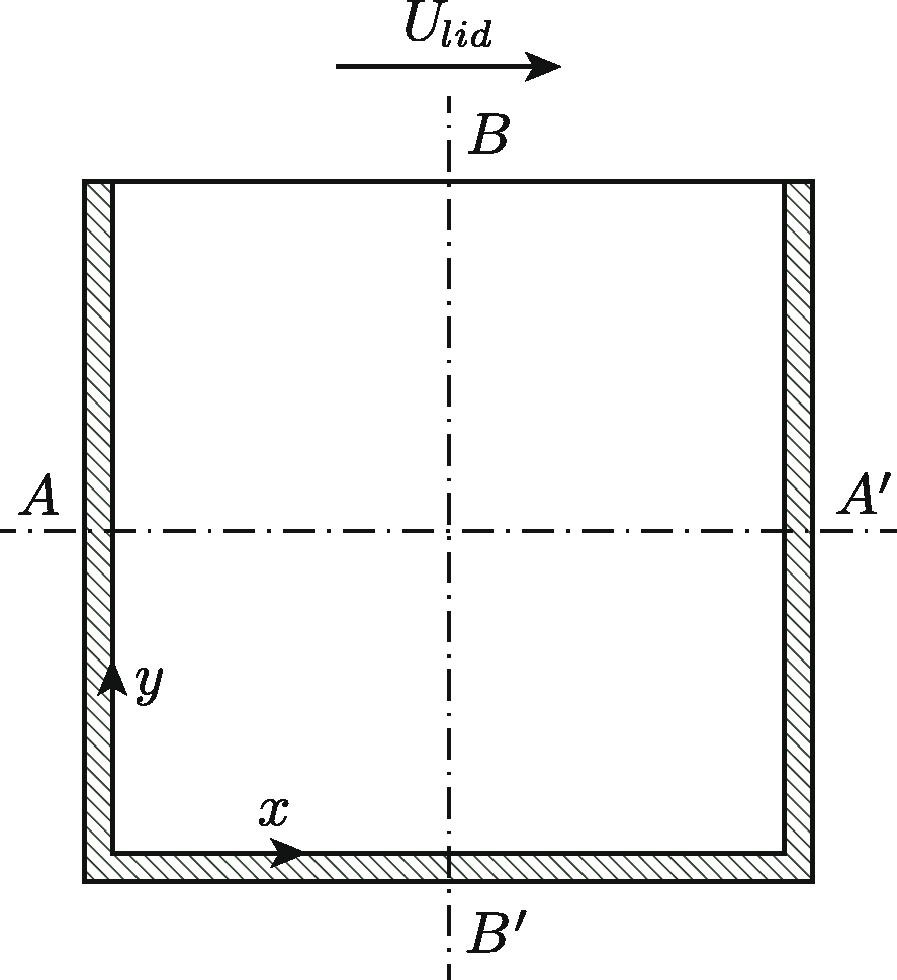
\includegraphics[width=.6\columnwidth]{cnrs-geometry}
	\caption{2m$\times$2m 2D domain of the CNRS Benchmark. $U_{lid}$
	represents the velocity along the top boundary. For comparison, various quantities are
	measured along the centerlines AA' and BB'. From Tiberga et
	al. \cite{tiberga_results_2020}.}
	\label{fig:cnrs-geometry}
\end{figure}

As shown in Figure \ref{fig:cnrs-geometry}, the domain geometry is a
2m$\times$2m square cavity filled with LiF-BeF$_2$-UF$_4$ molten salt at an
initial temperature of 900K \cite{tiberga_results_2020}.
Standard vacuum boundary conditions apply for neutron flux along all
boundaries whereby outgoing neutrons are considered lost, while homogeneous
boundary conditions apply for delayed neutron precursors. No-slip boundary
conditions apply for velocity variables in the cavity, except along the top
boundary for Steps 0.1, 0.3, 1.1, 1.2, and 1.4, which impose forced flow in the
form of lid-driven
cavity flow. For the temperature variable, all boundaries are insulated, and we
simulate salt cooling with the following volumetric heat sink equation:
%
\begin{align}
    q'''(\vec{r}) &= \gamma \left(900 - T(\vec{r})\right) \label{eq:cnrs-heat}
    \shortintertext{where}
    q''' &= \mbox{volumetric heat sink [W$\cdot$m$^{-3}$],}
    \nonumber \\
    \gamma &= \mbox{heat transfer coefficient [W$\cdot$m$^{-3}\cdot$K$^{-1}$],}
    \nonumber \\
    T(\vec{r}) &= \mbox{temperature at point $\vec{r}$ [K].} \nonumber
\end{align}

Tiberga et al. \cite{tiberga_results_2020} used Serpent 2
\cite{leppanen_serpent_2014} with the JEFF-3.1 library
\cite{koning_jeff-31_2006} to generate multigroup neutronics data for the
LiF-BeF$_2$-UF$_4$ salt in the domain at 900K, which they condensed into six
energy groups and eight precursor groups. We direct readers to their paper for
the group constant data \cite{tiberga_results_2020}. In addition, the
benchmark prescribes the following equations to govern the temperature
dependence in the cross sections and the neutron diffusion coefficients:
%
\begin{align}
    \Sigma_i (T) &= \Sigma_i(T_{ref})
    \frac{\rho_{fuel}(T)}{\rho_{fuel}(T_{ref})}
    \shortintertext{and}
    D (T) &= D(T_{ref})
    \frac{\rho_{fuel}(T_{ref})}{\rho_{fuel}(T)}
    \shortintertext{where}
    \Sigma_i &= \mbox{relevant macroscopic cross section [cm${-1}$],}
    \nonumber \\
    D &= \mbox{neutron diffusion coefficient [cm$^2\cdot$s$^{-1}$],}   
    \nonumber \\
    \rho_{fuel} &= \mbox{density of the fuel salt [kg$\cdot$m$^{-3}$],}
    \nonumber \\
    T_{ref} &= \mbox{reference temperature} = 900\mbox{ K}. \nonumber
\end{align}

The benchmark also prescribes incompressible Navier-Stokes flow with the
Boussinesq approximation for evaluating the salt flow in the
domain but does not restrict the type of neutronics model.
Table \ref{table:benchmark} lists the relevant input parameters and observables.

\begin{table*}[tp!]
	\caption{Input parameters and observables of each benchmark step.}
	\centering
	\footnotesize
    \begin{tabular}{p{.05\textwidth} p{.1\textwidth} p{.3\textwidth} p{.45\textwidth}}
		\toprule
        \textbf{Step} & \textbf{Name} & \textbf{Input parameters} & \textbf{Observables} \\
		\midrule
        0.1 & Velocity field &
		\begin{itemize}[nosep,noitemsep,left=0pt,
		                before={\begin{minipage}[t]{\hsize}},
                        after ={\end{minipage}}]
		    \item $U_{lid} = 0.5$ m$\cdot$s$^{-1}$
		\end{itemize}\vspace*{-\baselineskip}\mbox{} &
		\begin{itemize}[nosep,noitemsep,left=0pt,
		                before={\begin{minipage}[t]{\hsize}},
                        after ={\end{minipage}}]
		    \item Velocity components $(u_x,u_y)$ along AA' and BB'
		\end{itemize}\vspace*{-\baselineskip}\mbox{} \\
        \midrule
        0.2 & Neutronics &
        \begin{itemize}[nosep,noitemsep,left=0pt,
		                before={\begin{minipage}[t]{\hsize}},
                        after ={\end{minipage}}]
		    \item $U_{lid} = 0$ m$\cdot$s$^{-1}$
		    \item $T = 900$ K
		    \item $P = 1$ GW
		\end{itemize} &
		\begin{itemize}[nosep,noitemsep,left=0pt,
		                before={\begin{minipage}[t]{\hsize}},
                        after ={\end{minipage}}]
		    \item Fission rate density $\sum^6_g \Sigma_{f,g} \phi_g(\vec{r})$ along AA'
            \item Reactivity $\rho$
		\end{itemize}\vspace*{-\baselineskip}\mbox{} \\
        \midrule
        0.3 & Temperature &
        \begin{itemize}[nosep,noitemsep,left=0pt,
		                before={\begin{minipage}[t]{\hsize}},
                        after ={\end{minipage}}]
		    \item Fixed flow field from Step 0.1 for
		    $U_{lid} = 0.5$ m$\cdot$s$^{-1}$
		    \item Fixed heat source distribution
		    $\sum^6_{g} \epsilon_g \Sigma_{f,g} \phi_g(\vec{r})$ from Step 0.2
		    \item $\gamma = 10^6$ W$\cdot$m$^{-3}\cdot$K$^{-1}$
		\end{itemize} &
		\begin{itemize}[nosep,noitemsep,left=0pt,
		                before={\begin{minipage}[t]{\hsize}},
                        after ={\end{minipage}}]
		    \item Temperature $T$ along AA' and BB'
		\end{itemize}\vspace*{-\baselineskip}\mbox{} \\
        \midrule
        1.1 & Circulating fuel &
        \begin{itemize}[nosep,noitemsep,left=0pt,
		                before={\begin{minipage}[t]{\hsize}},
                        after ={\end{minipage}}]
		    \item Fixed flow field from Step 0.1 for
		    $U_{lid} = 0.5$ m$\cdot$s$^{-1}$
		    \item $T = 900$ K
		    \item $P = 1$ GW
		\end{itemize} &
		\begin{itemize}[nosep,noitemsep,left=0pt,
		                before={\begin{minipage}[t]{\hsize}},
                        after ={\end{minipage}}]
		    \item Delayed neutron source $\sum^8_i \lambda_i C_i$ along AA' and BB'
		    \item Reactivity change between Step 1.1 and Step 0.2,
		    $\Delta \rho = \rho - \rho_{s_{0.2}}$
		\end{itemize}\vspace*{-\baselineskip}\mbox{} \\
        \midrule
        1.2 & Power coupling &
        \begin{itemize}[nosep,noitemsep,left=0pt,
		                before={\begin{minipage}[t]{\hsize}},
                        after ={\end{minipage}}]
		    \item Fixed flow field from Step 0.1 for
		    $U_{lid} = 0.5$ m$\cdot$s$^{-1}$
		    \item $P = 1$ GW
		    \item $\gamma = 10^6$ W$\cdot$m$^{-3}\cdot$K$^{-1}$
		\end{itemize}\vspace*{-\baselineskip}\mbox{} &
		\begin{itemize}[nosep,noitemsep,left=0pt,
		                before={\begin{minipage}[t]{\hsize}},
                        after ={\end{minipage}}]
		    \item Temperature $T$ along AA' and BB'
            \item Reactivity change between Step 1.2 and Step 1.1,
            $\Delta\rho = \rho - \rho_{s_{1.1}}$
            \item Change in fission rate density
            $\sum^6_g \Sigma_{f,g} \phi_g(\vec{r}) -
            \left[\sum^6_g \Sigma_{f,g} \phi_g(\vec{r})\right]_{s_{0.2}}$
		\end{itemize} \\
        \midrule
        1.3 & Buoyancy &
        \begin{itemize}[nosep,noitemsep,left=0pt,
		                before={\begin{minipage}[t]{\hsize}},
                        after ={\end{minipage}}]
		    \item $P = 1$ GW
		    \item $U_{lid} = 0$ m$\cdot$s$^{-1}$
		    \item $\gamma = 10^6$ W$\cdot$m$^{-3}\cdot$K$^{-1}$
		\end{itemize}\vspace*{-\baselineskip}\mbox{} &
		\begin{itemize}[nosep,noitemsep,left=0pt,
		                before={\begin{minipage}[t]{\hsize}},
                        after ={\end{minipage}}]
		    \item Velocity components $(u_x, u_y)$ along AA' and BB'
            \item Temperature $T$ along AA' and BB'
            \item Delayed neutron source $\sum^8_i \lambda_i C_i$ along AA' and BB'
            \item Reactivity change from Step 0.2
        $\Delta\rho = \rho - \rho_{s_{0.2}}$
		\end{itemize} \\
        \midrule
        1.4 & Full coupling &
        \begin{itemize}[nosep,noitemsep,left=0pt,
		                before={\begin{minipage}[t]{\hsize}},
                        after ={\end{minipage}}]
		    \item $\gamma = 10^6$ W$\cdot$m$^{-3}\cdot$K$^{-1}$
		    \item $P$ variable in the range $[0,1]$ GW with a step of 0.2 GW
		    \item $U_{lid}$ variable in the range $[0,0.5]$ m$\cdot$s$^{-1}$
		    with a step of 0.1 m$\cdot$s$^{-1}$
		\end{itemize} &
		\begin{itemize}[nosep,noitemsep,left=0pt,
		                before={\begin{minipage}[t]{\hsize}},
                        after ={\end{minipage}}]
		    \item Reactivity change between Step 1.4 and Step 0.2,
		    $\Delta\rho = \rho - \rho_{s_{0.2}}$, for all permutations of $P$
		    and $U_{lid}$ values
		\end{itemize}\vspace*{-\baselineskip}\mbox{} \\
        \midrule
        2.1 & Forced convection transient &
        \begin{itemize}[nosep,noitemsep,left=0pt,
		                before={\begin{minipage}[t]{\hsize}},
                        after ={\end{minipage}}]
		    \item $\gamma = 10^6$ W$\cdot$m$^{-3}\cdot$K$^{-1}$
            \item Steady-state solution from Step 1.4 for $U_{lid} = 0.5$
        m$\cdot$s$^{-1}$ and $P = 1.0$ GW
		\end{itemize} &
		\begin{itemize}[nosep,noitemsep,left=0pt,
		                before={\begin{minipage}[t]{\hsize}},
                        after ={\end{minipage}}]
		    \item Power gain and shift as a function of the perturbation frequency
		\end{itemize}\vspace*{-\baselineskip}\mbox{} \\
		\bottomrule
	\end{tabular}
	\label{table:benchmark}
\end{table*}

Step 2.1 studies the transient response of the fully coupled nonlinear system.
Linear perturbation analyses are performed by introducing periodic
perturbations to the heat transfer coefficient $\gamma$ and studying the gain
and phase shift of the response in the total power $P$. For the initial
conditions, the steady-state solution from Step 1.4 with
$U_{lid} = 0.5$ m$\cdot$s$^{-1}$ and $P = 1$ GW is used. This initial
configuration is made exactly critical by scaling the neutron source terms,
from fission and \gls{DNP} decay, by the inverse of the criticality eigenvalue
solution from Step 1.4.

$\gamma$ is uniformly perturbed according to small-amplitude sine waves given
as:
%
\begin{align}
    \gamma =& \gamma_0 \left[ 1 + 0.1\sin\left(2 \pi f \right) \right]
    \shortintertext{where}
    \gamma_0 =& 10^6 \mbox{ W$\cdot$m$^{-3}\cdot$K$^{-1}$}, \nonumber \\
    f \in& \left\lbrace 0.0125, 0.025, 0.05, 0.1, 0.2, 0.4, 0.8 \right\rbrace 
    \mbox{ Hz.} \nonumber
\end{align}

The benchmark defines power gain as:
%
\begin{align}
    \mbox{Power gain} =& \frac{\left(P_{max} - P_{avg}\right)/P_{avg}}{
    \left(\gamma_{max} - \gamma_{avg}\right)/\gamma_{avg}}
\end{align}
%
The subscripts denote the maximum and time-averaged values of $P$ and $\gamma$.

\FloatBarrier

\subsection{Modeling Approach with Moltres} \label{sec:model}

This section describes the specific modeling approach for
simulating the CNRS Benchmark cases in Moltres.

For this work\footnote{The input files for
all benchmark
cases are available on the Moltres GitHub repository at 
\url{https://github.com/arfc/moltres/tree/devel/problems/2021-cnrs-benchmark}.
}, I ran the benchmark cases on a uniformly-spaced mesh
of 200$\times$200 elements. Thus, the dimensions of each mesh element are
0.01m$\times$0.01m. I adopted the group constant data
provided by Tiberga et al. \cite{tiberga_results_2020}. Next, I
discretized most variables, i.e., neutron fluxes, velocity
components, pressure, and temperature, using continuous, first-order, Lagrange
shape functions. The only exception is the precursor concentration variables,
which I discretized using zeroth-order monomial shape functions and solved
using a \gls{DFEM}. I interpolated the resulting discontinuous,
cell-centered precursor values to obtain the nodal values for results
analysis.

The
\texttt{Navier-Stokes} and \texttt{Heat} \texttt{Conduction} modules from
\gls{MOOSE} provide some of the capabilities for
modeling incompressible flow and heat transfer. In particular, I stabilized
the incompressible flow and temperature governing equations using the
\gls{SUPG} stabilization method implemented in \gls{MOOSE}
\cite{peterson_overview_2018}. Without \gls{SUPG} stabilization, I
observed spurious numerical oscillations in the velocity and temperature near
the top boundary due to the singularity on the top left corner where different
velocity boundary conditions meet. I also applied the \gls{PSPG} stabilization
scheme \cite{hughes_new_1986} from the Navier-Stokes module
\cite{peterson_overview_2018},
which enables equal-order discretizations in the velocity and pressure
variables. Equal-order discretizations with \gls{PSPG} are computationally
cheaper and more convenient than implementing higher-order
velocity discretizations for stability without \gls{PSPG}
\cite{chapelle_inf-sup_1993}.

Using the inverse power method solver in \gls{MOOSE}, I ran all eigenvalue calculations in
Steps 0.2, 1.1, 1.2, 1.3, and 1.4. I ran all other steps
using the Preconditioned Newton-Krylov solver
\cite{gaston_physics-based_2015}. The coupled steady-state problems in
Steps 1.2, 1.3, and 1.4 required segregated solvers for the neutronics
and the thermal-hydraulics due to the unique problem setups involving a
criticality search problem for the neutron multiplication factor
and a steady-state problem in thermal-hydraulics simultaneously.

\begin{table}[tb]
    \caption{Timestep sizes used for the time-dependent cases in
    Step 2.1, corresponding to 1/200th of the perturbation period.}
	\centering
	\setlength\tabcolsep{2.5pt}
	\begin{tabular}{l l l l l l l l}
	    \toprule
	    Frequency [Hz] & 0.0125 & 0.025 & 0.05 & 0.1 & 0.2 & 0.4 & 0.8 \\
	    \midrule
	    Timestep size [s] & 0.2 & 0.2 & 0.1 & 0.05 & 0.025 & 0.0125 & 0.00625
	    \\
	    \bottomrule
	\end{tabular}
	\label{table:timestep}
\end{table}

For the time-dependent cases in Step 2.1, I employed full coupling with
a second-order implicit Backward Differential Formula (BDF2) time-stepping
scheme. I set the timestep sizes for each driving frequency in the heat transfer
coefficient to 1/200th of the perturbation period. Table
\ref{table:timestep} shows the timestep sizes. I assumed the
systems reached asymptotic behavior when the magnitudes of neighboring power
peaks differed by less than 0.001\% for at least ten wavelengths. Under this
assumption, the phase shift measurements between adjacent waves always
converged before the magnitude measurements of the power peaks.

Table \ref{table:software} compares the numerical methods, meshing schemes, and
neutronics models of Moltres and the four participating software packages in
the CNRS benchmark paper \cite{tiberga_results_2020}. The $SP_N$ and
$S_N$ neutronics models refer to the simplified $P_N$ spherical harmonics and
$S_N$ discrete ordinates neutron transport models, respectively. Based on the
solvers and methods of solution, Moltres is most similar to the
PHANTOM-$S_N$ + DGFlows \cite{tiberga_discontinuous_2019} multiphysics package
from \gls{TUD} with the $S_2$ neutron transport model. Participants from
\gls{CNRS} and \gls{PSI}
employed non-uniform meshes which were refined near the boundaries. In contrast,
we and the \gls{PoliMi} and \gls{TUD} participants employed uniform meshes.

\FloatBarrier

\begin{landscape}
\begin{table*}[p]
    \caption{List of software packages and their corresponding model
    specifications for the CNRS Benchmark simulations
    \cite{tiberga_results_2020}.}
    \centering
    \begin{tabular}{p{4.2cm} p{7cm} p{3.3cm} p{2cm} p{2.7cm}}
        \toprule
        Software & Institute & Numerical method & Mesh & Neutronics model \\
        \midrule
        OpenFOAM & Centre national de la recherche scientifique (CNRS) & Finite volume & 200$\times$200 \newline Non-uniform & $SP_1$ \& $SP_3$ \\
        OpenFOAM & Politecnico di Milano (PoliMi) & Finite volume & 400$\times$400 \newline Uniform & Neutron diffusion \\
        GeN-Foam & Paul Scherrer Institute (PSI) & Finite volume & 200$\times$200 \newline Non-uniform & Neutron diffusion \\
        PHANTOM-$S_N$+DGFlows & Delft University of Technology (TUD) & Discontinuous finite \newline element & 50$\times$50 \newline Uniform & $S_2$ \& $S_6$ \\
        Moltres (This work) & University of Illinois at Urbana-Champaign (UIUC) & Continuous \& discontinuous finite element & 200$\times$200 \newline Uniform & Neutron diffusion \\
        \bottomrule
    \end{tabular}
    \label{table:software}
\end{table*}
\end{landscape}

\FloatBarrier

\subsection{Results \& Discussion}

In this section, we compare the results from Moltres for each CNRS Benchmark
step to the results in the benchmark paper \cite{tiberga_results_2020}.
The software packages from \gls{CNRS} and \gls{TUD}
each report two sets of results from different angular discretizations
in their neutronics models for Steps 0.2, 1.1, 1.2, 1.3, 1.4, and 2.1. These
sets of results are labeled as CNRS-$SP_1$ and
CNRS-$SP_3$; and TUD-$S_2$ and TUD-$S_6$, respectively. The
authors performed code-to-code verification by sampling observable values at
201 equidistant points along the centerlines AA' and BB' and reporting the
discrepancy $\epsilon_c$ of each observable from each software
(indexed by $c$) for each measured observable $Q_c$ (not to be confused with
fission heat source $Q_f$), relative to the average of
that same observable $Q_{avg}$ from all participating software. Variables
$\epsilon_c$ and $Q_{avg}$ are calculated as:
%
\begin{align}
    \epsilon_c =& \sqrt{\frac{\sum^{N_p}_{i=1}\left[Q_c(\vec{r_i}) - Q_{avg}
    (\vec{r_i})\right]^2}{\sum^{N_p}_{i=1} Q^2_{avg}(\vec{r_i})}}
    \shortintertext{and}
    Q_{avg}(\vec{r_i}) =& \frac{1}{N_c} \sum^{N_c}_{c=1} Q_c(\vec{r_i})
    \shortintertext{where}
    Q_c(\vec{r_i}) =&
    \mbox{ value of observable $Q$ at location $\vec{r_i}$ from software $c$,}
    \nonumber \\
    N_p =& \mbox{ number of sampling points of quantity $Q$} = 201,
    \nonumber \\
    N_c =& \mbox{ number of participating software packages.} \nonumber
\end{align}

The average discrepancy $\epsilon$ across all software is calculated as:
%
\begin{align}
    \epsilon =& \frac{1}{N_c}\sum^{N_c}_{c=1} \epsilon_c
\end{align}

We adopted the averaged values $\epsilon$ and $Q_{avg}$ directly from the
reference work \cite{tiberga_results_2020} without including our results
in the calculations. We note that the benchmark does not provide a reference
solution, and a significantly erroneous value from one of the software packages
could heavily skew the discrepancy values. Nevertheless, the benchmark paper
reports good agreement among their software packages.

For observables measured along the centerlines AA' and BB', Tables
\ref{table:disc0} and \ref{table:disc1} report the discrepancy $\epsilon_c$ of
each observable from Moltres relative to the average of the benchmark
participants $Q_{avg}$ alongside the average discrepancy $\epsilon$ of
the benchmark participants. We also reproduce corresponding plots
in the benchmark paper for every observable along AA' or BB' in Figures
\ref{fig:0.1}, \ref{fig:0.2}, \ref{fig:0.3}, \ref{fig:1.1}, \ref{fig:1.2},
\ref{fig:1.3}, and \ref{fig:2.1} for a qualitative comparison of the results
from Moltres and the benchmark participants. Given the significant overlap in
the plot curves, these figures omit results from CNRS-$SP_1$ and TUD-$S_2$ to
reduce cluttering. The full dataset
of all observable results used in this results analysis is
available at \cite{park_results_2021}. Lastly, Table
\ref{table:rho} reports all reactivity and reactivity changes from
Steps 0.2, 1.1, 1.2, and 1.3.

\begin{figure}[h]
	\centering
    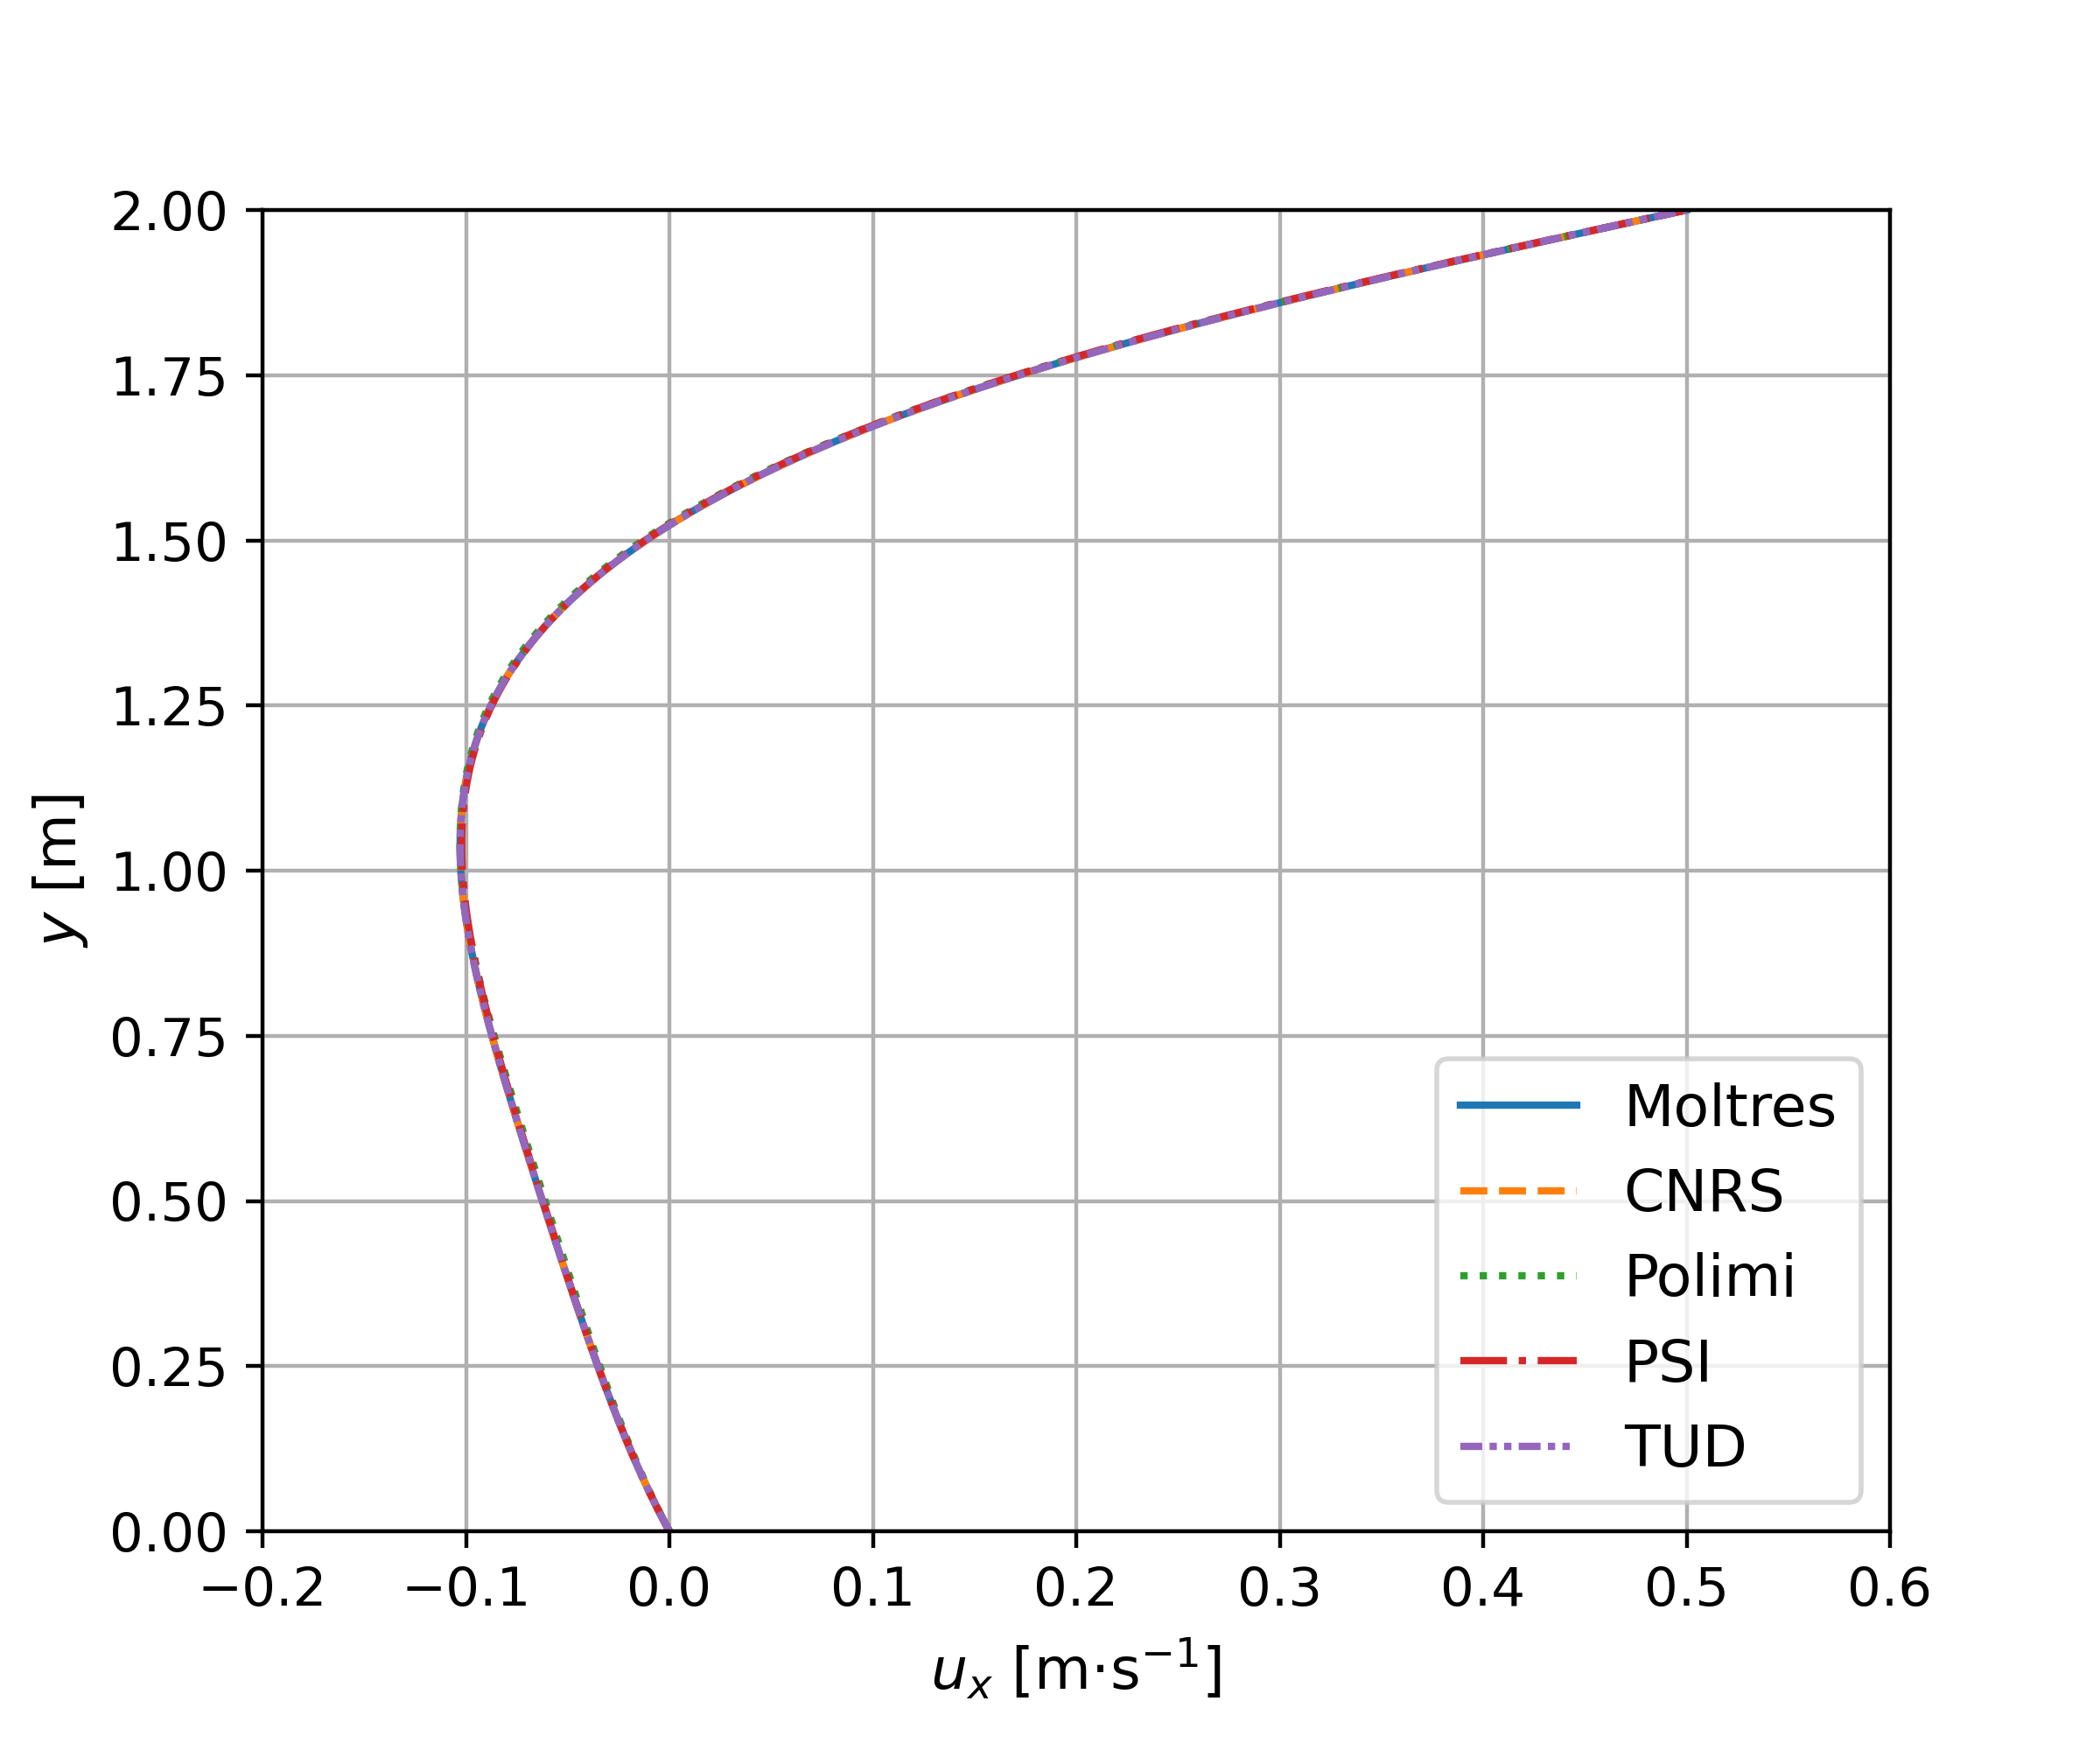
\includegraphics[width=.49\columnwidth]{0-1-vel-plot}
	\caption{Step 0.1 \textemdash\ Horizontal velocity component along BB'.}
	\label{fig:0.1}
\end{figure}
%
\begin{figure}[h]
	\centering
    \begin{subfigure}[b]{.49\textwidth}
      \centering
	  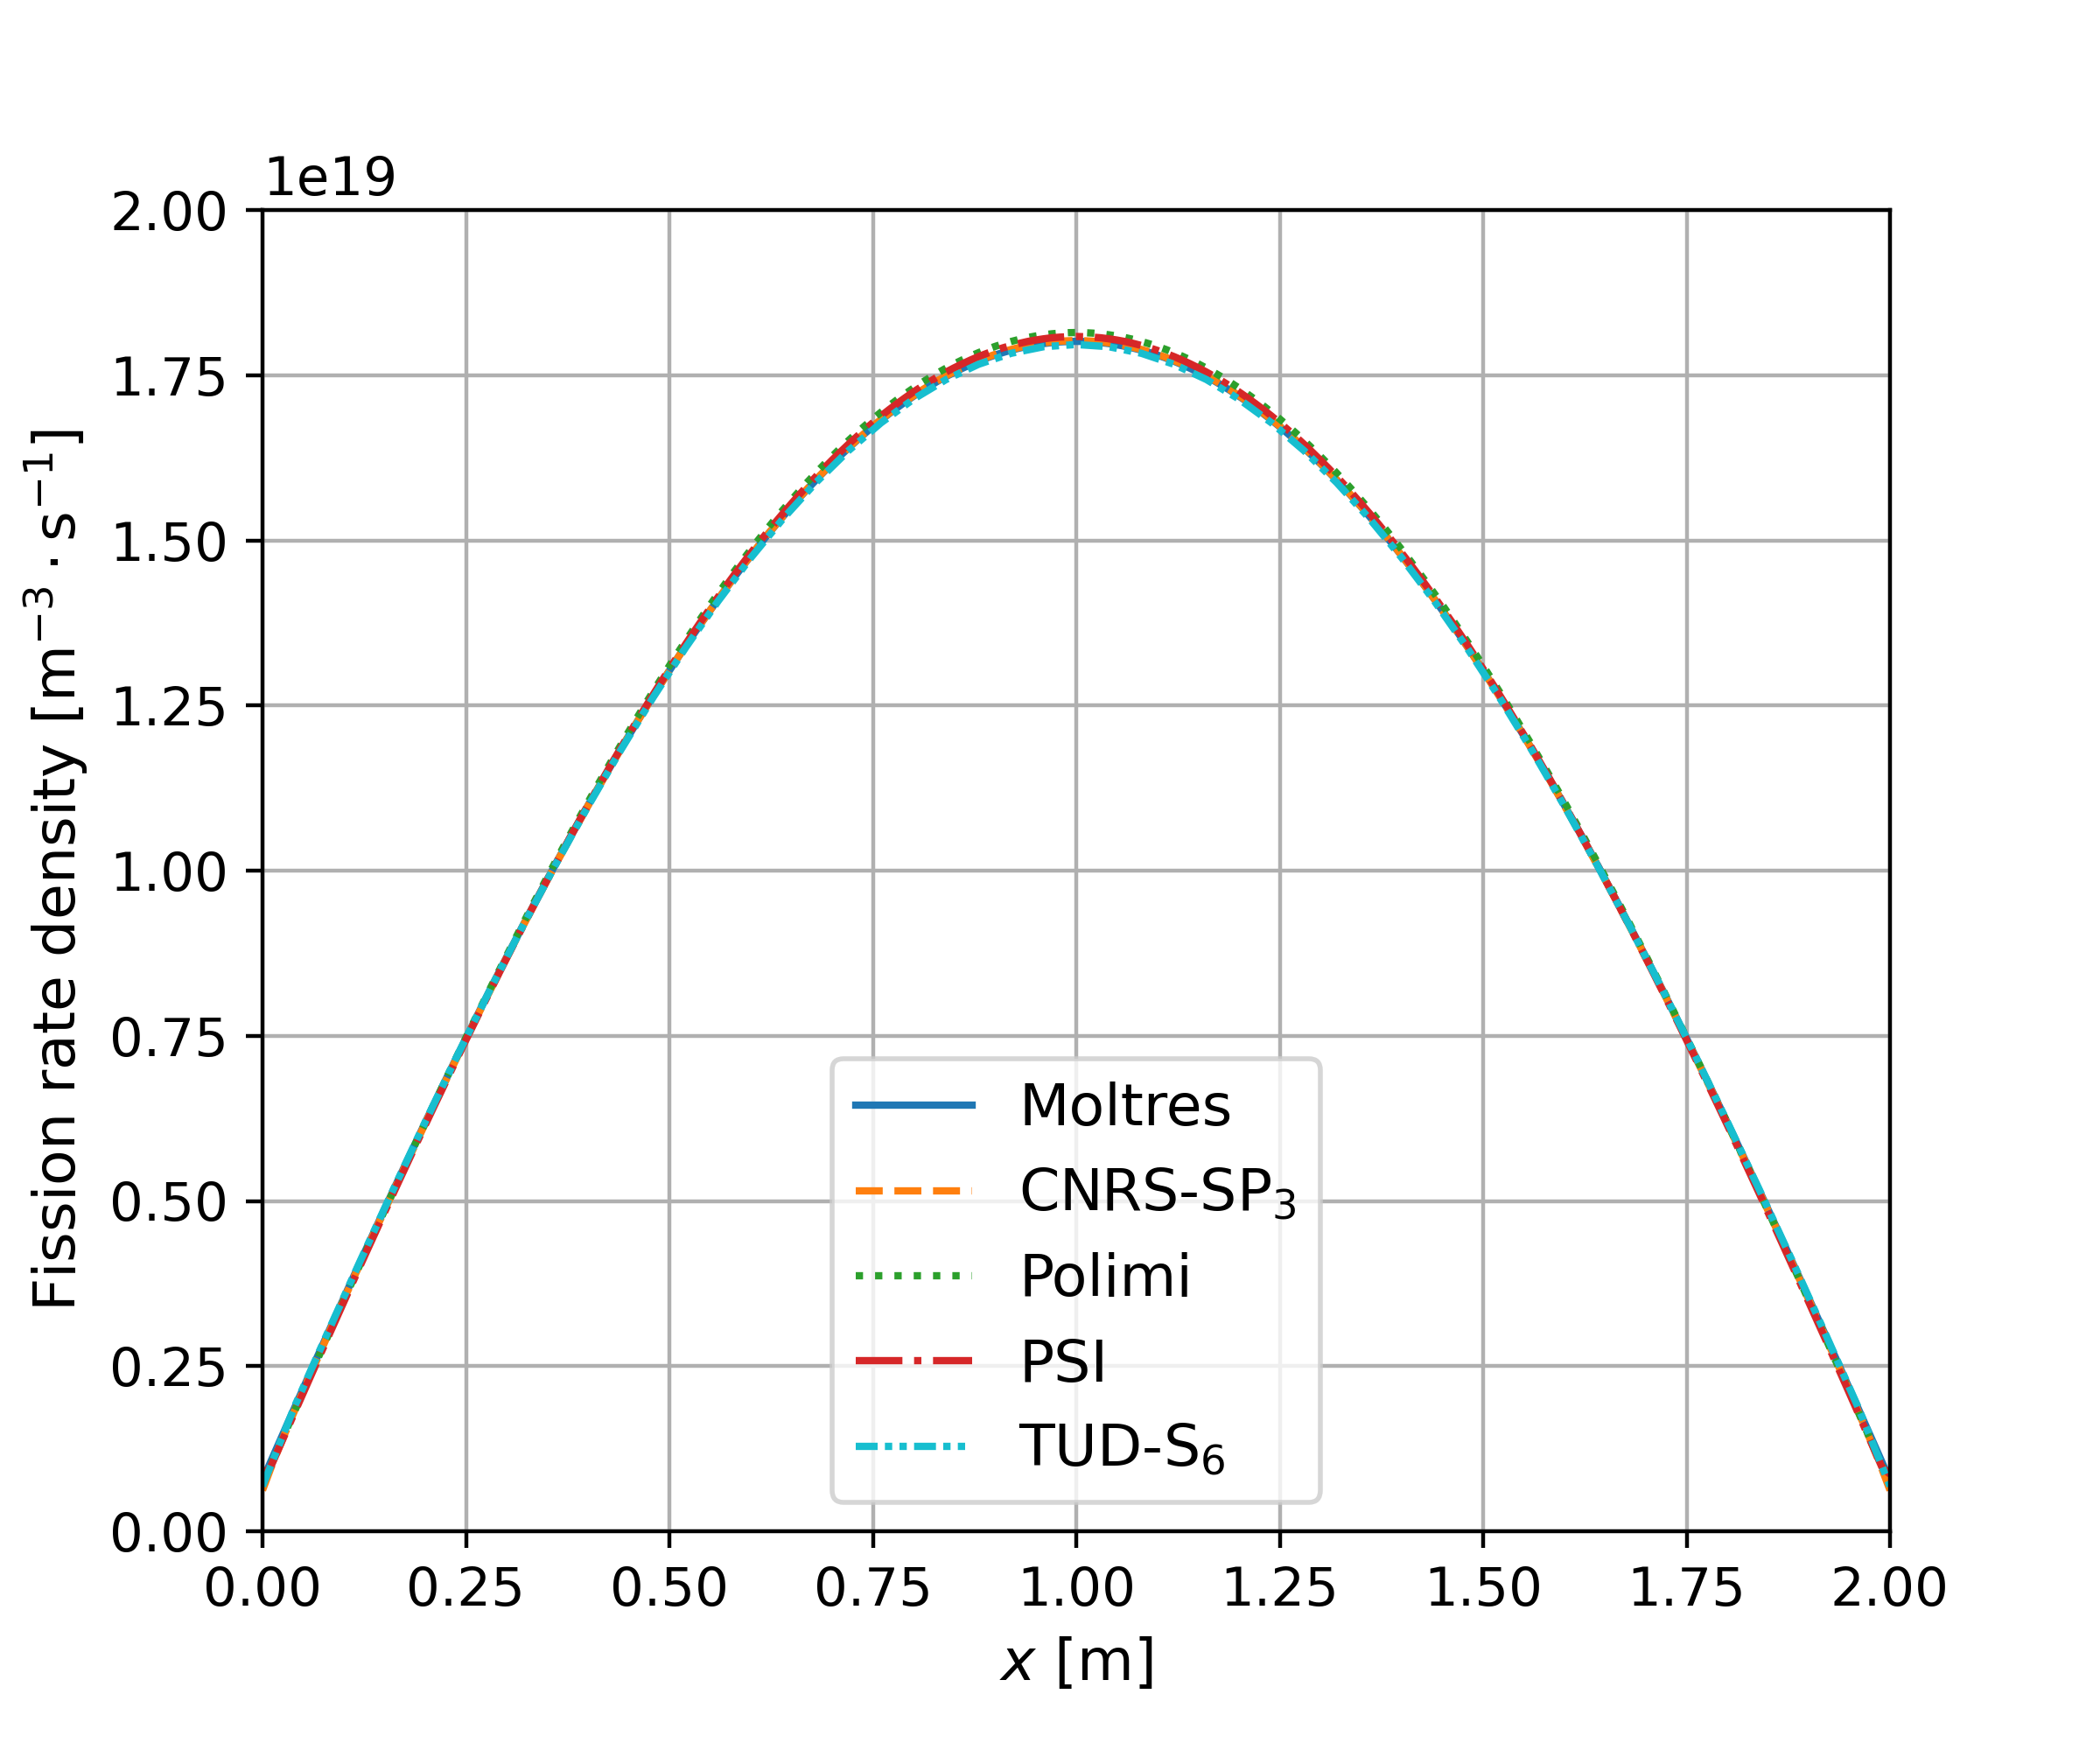
\includegraphics[width=\columnwidth]{0-2-fiss-plot}
	  \caption{Step 0.2 \textemdash\ Fission rate density along AA'.}
	  \label{fig:0.2}
    \end{subfigure}
    \hfill
    \begin{subfigure}[b]{.49\textwidth}
      \centering
	  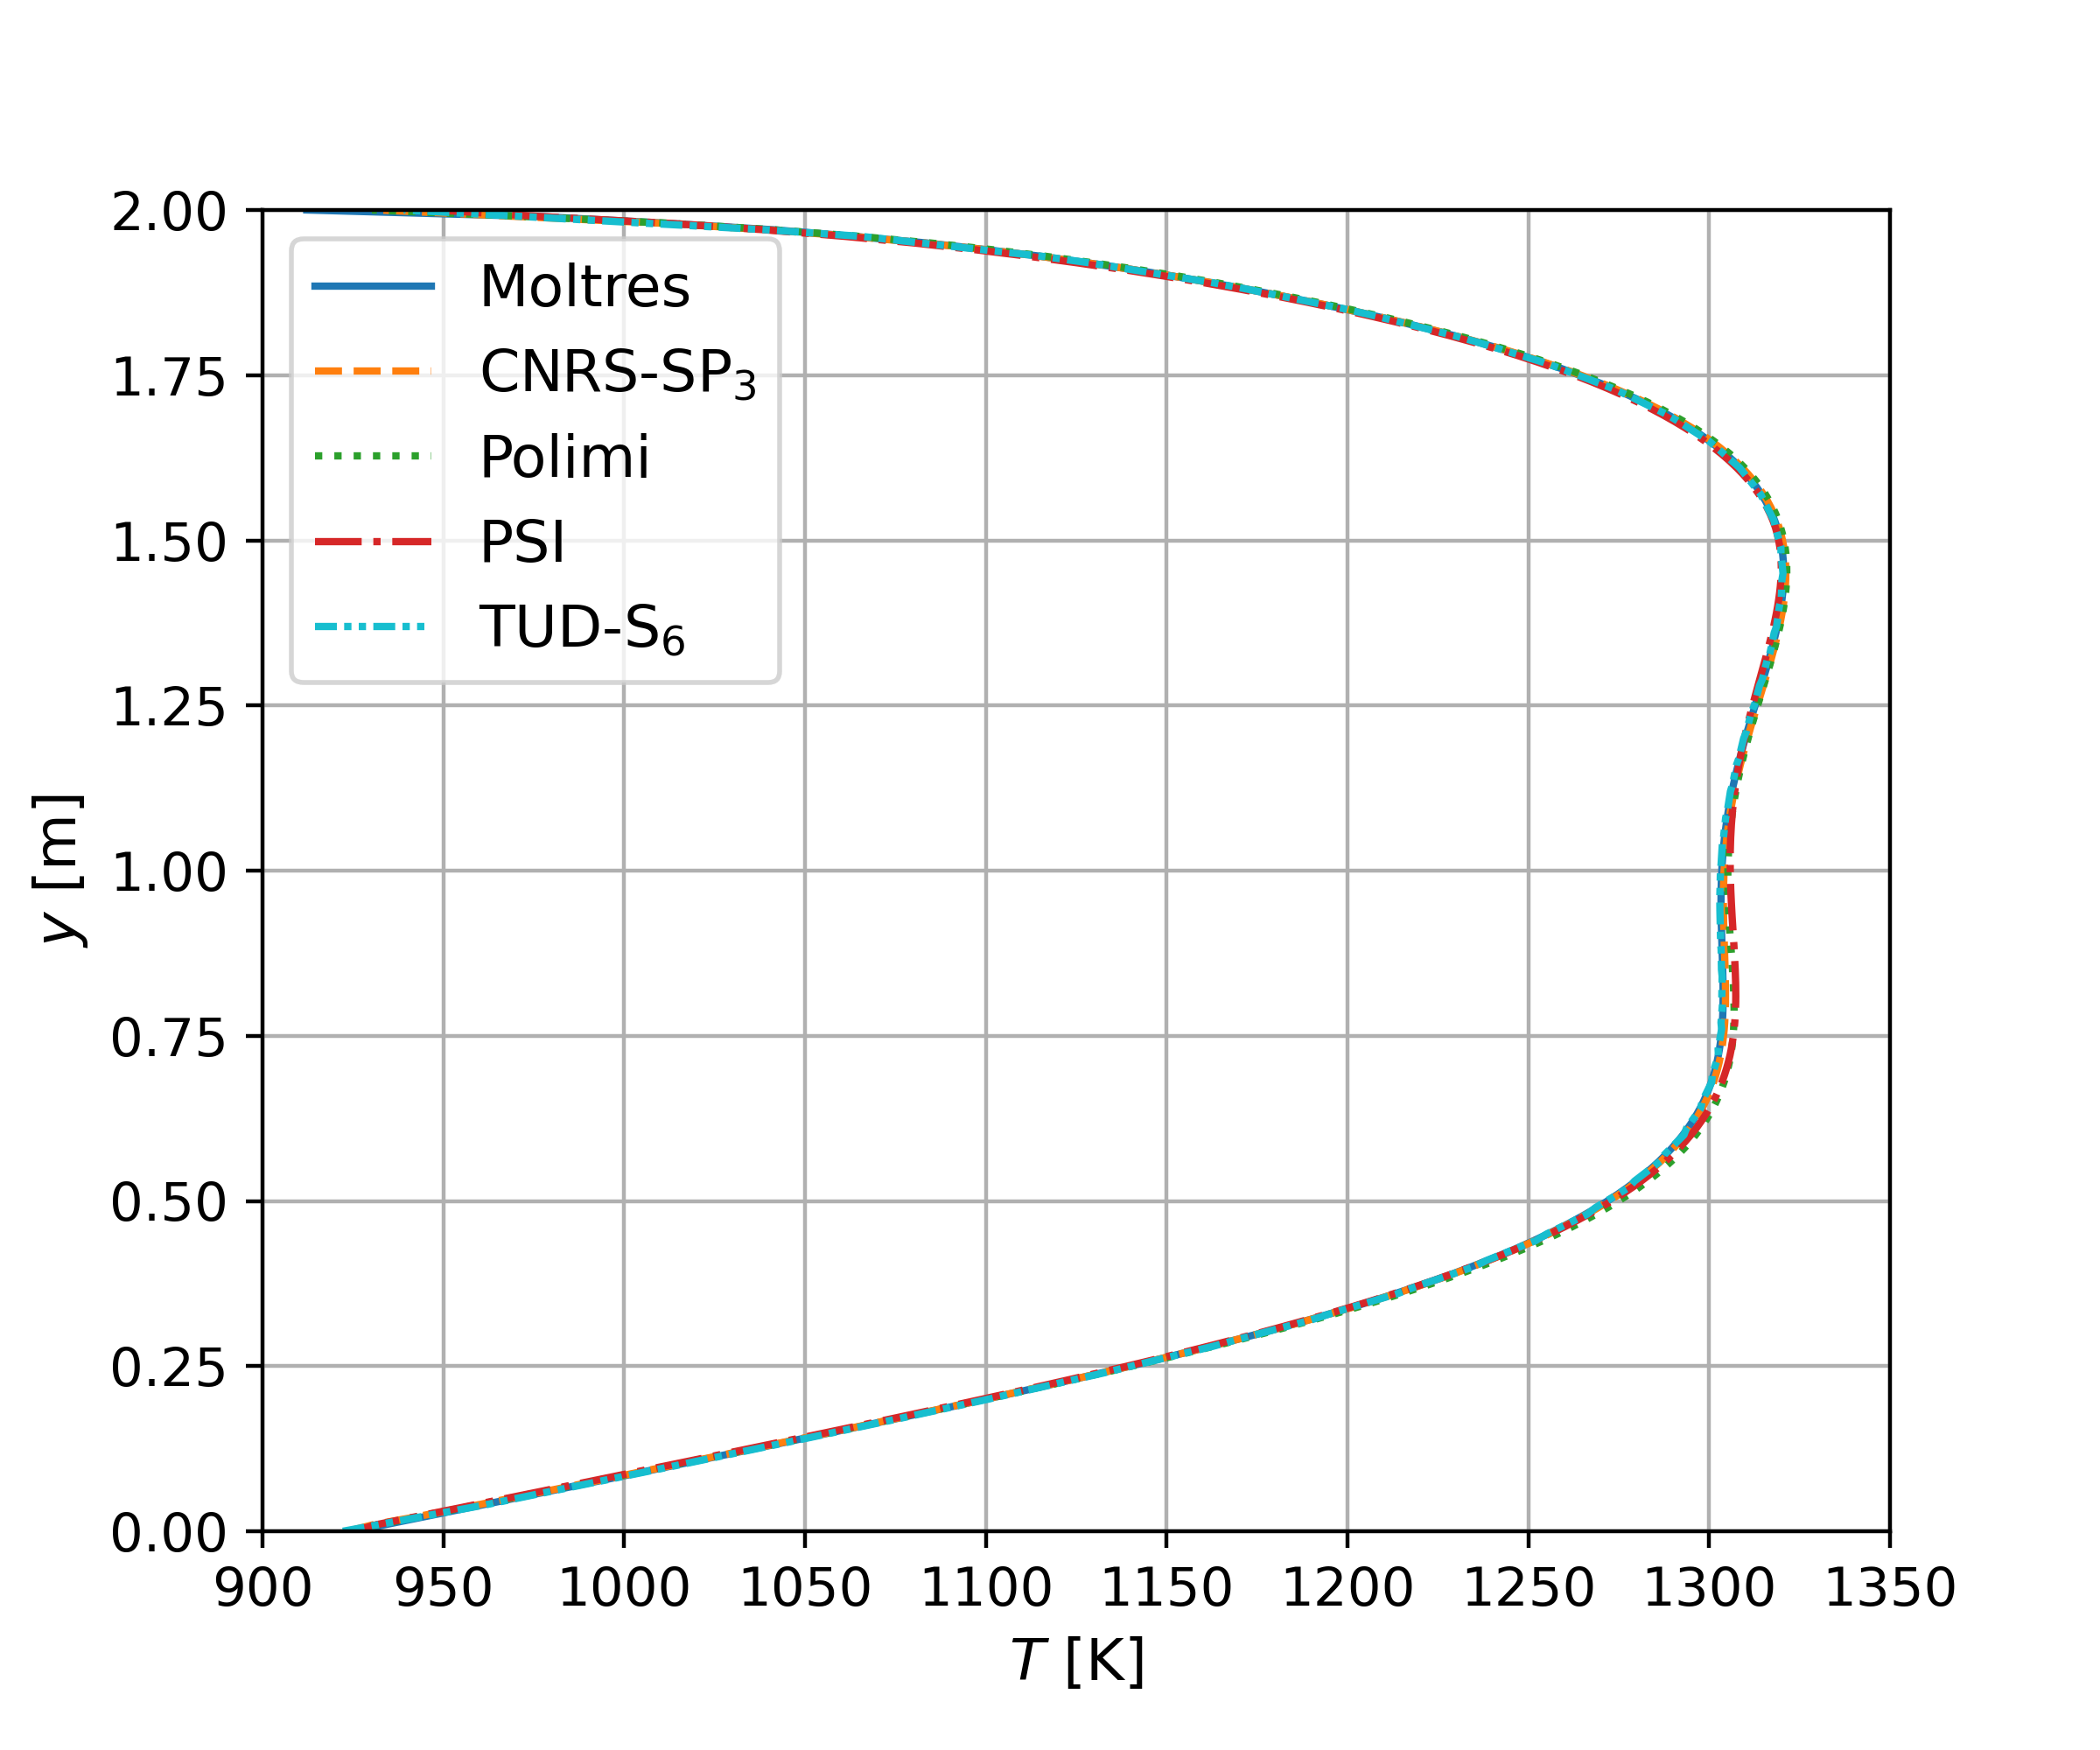
\includegraphics[width=\columnwidth]{0-3-temp-plot}
	  \caption{Step 0.3 \textemdash\ Temperature distribution along BB'.}
	  \label{fig:0.3}
    \end{subfigure}
\end{figure}
%
\FloatBarrier
%
\begin{table}[htb]
	\caption{Discrepancy values from Moltres alongside the average and standard
	deviation of the discrepancy values of the benchmark participants for Phase
	0.}
	\centering
	\small
	\begin{tabular}{l l c S S S}
		\toprule
		\multirow{2}{*}{\textbf{Step}} & \multirow{2}{*}{\textbf{Observable}} & \multirow{2}{*}{\textbf{Centerline}} & {\multirow{2}{*}{\textbf{Moltres [\%]}}} & \multicolumn{2}{c}{\textbf{Benchmark [\%]}} \\
		& & & & {Average} & {SD} \\
		\midrule
		\multirow{4}{*}{0.1} &
		\multirow{2}{*}{$u_x$} & AA' & 0.247 & 0.253 & 0.150 \\
		& & BB' & 0.266 & 0.318 & 0.102 \\
		\cmidrule{2-6}
		& \multirow{2}{*}{$u_y$} & AA' & 0.540 & 0.598 & 0.266 \\
		& & BB' & 0.468 & 0.795 & 0.421 \\
		\midrule
		{0.2} &
		{$\sum^6_g \Sigma_{f,g} \phi_g(\vec{r})$} & AA' & 0.313 & 0.285 & 0.153
		\\
		\midrule
		\multirow{2}{*}{0.3} &
		\multirow{2}{*}{$T$} & AA' & 0.090 & 0.085 & 0.031 \\
		& & BB' & 0.164 & 0.083 & 0.027\\
		\bottomrule
	\end{tabular}
	\label{table:disc0}
\end{table}

\subsubsection{Phase 0 results \& discussion}

Figures \ref{fig:0.1}, \ref{fig:0.2}, and \ref{fig:0.3} show that Moltres
accurately reproduced all three sets of results in Phase 0 for the velocity
field, fission rate density, and temperature. Table
\ref{table:disc0} reports the discrepancy values from Moltres for Phase 0 and
the corresponding average and \gls{SD} of the discrepancy values from
the benchmark participants
\cite{tiberga_results_2020}. Moltres performs very well as most discrepancy
values are either lower than or fall within one \gls{SD} of the benchmark
average discrepancies. The discrepancy value for $T$ along centerline BB' in
Step 0.3 is the only exception, with its value of 0.164\% being larger than
the benchmark average by 3 \gls{SD}.

Figure \ref{fig:0.3} shows that the $T$ distribution from Moltres is almost
identical to the corresponding distributions from CNRS-$SP_3$ and TUD-$S_6$
along most of centerline BB'. However, Figure \ref{fig:0.3-zoom} shows a
significant spread in the $T$ distributions along BB' from all software
packages near the top boundary. At $y = 2.0$ m, Moltres underpredicts the
temperature at 912.3 K compared to the benchmark participants' values which
range between 930.3 K and 948.1 K. This point on the top boundary lies directly downstream of
the velocity boundary condition discontinuity at the top-left corner.
Corner singularities are generally tricky to approximate with
continuous Galerkin methods \cite{kuhlmann_lid-driven_2018}.
The \gls{SUPG} stabilization scheme dampens numerical oscillations by
introducing pointwise artificial thermal diffusivity, which depends strongly on
the inverse of local velocity magnitude \cite{peterson_overview_2018}.
Therefore, while the \gls{SUPG} scheme effectively eliminates
spurious numerical oscillations everywhere else, it provides little damping
along the top boundary due to the relatively large non-zero velocity boundary
condition. On the other hand, the temperature values in the rest of the domain
and the average discrepancies of the other variables show that Moltres can
still accurately reproduce the expected results, and the temperature deviations
along the top boundary do not impact the overall integrity of our results.

\begin{figure}[htb]
	\centering
	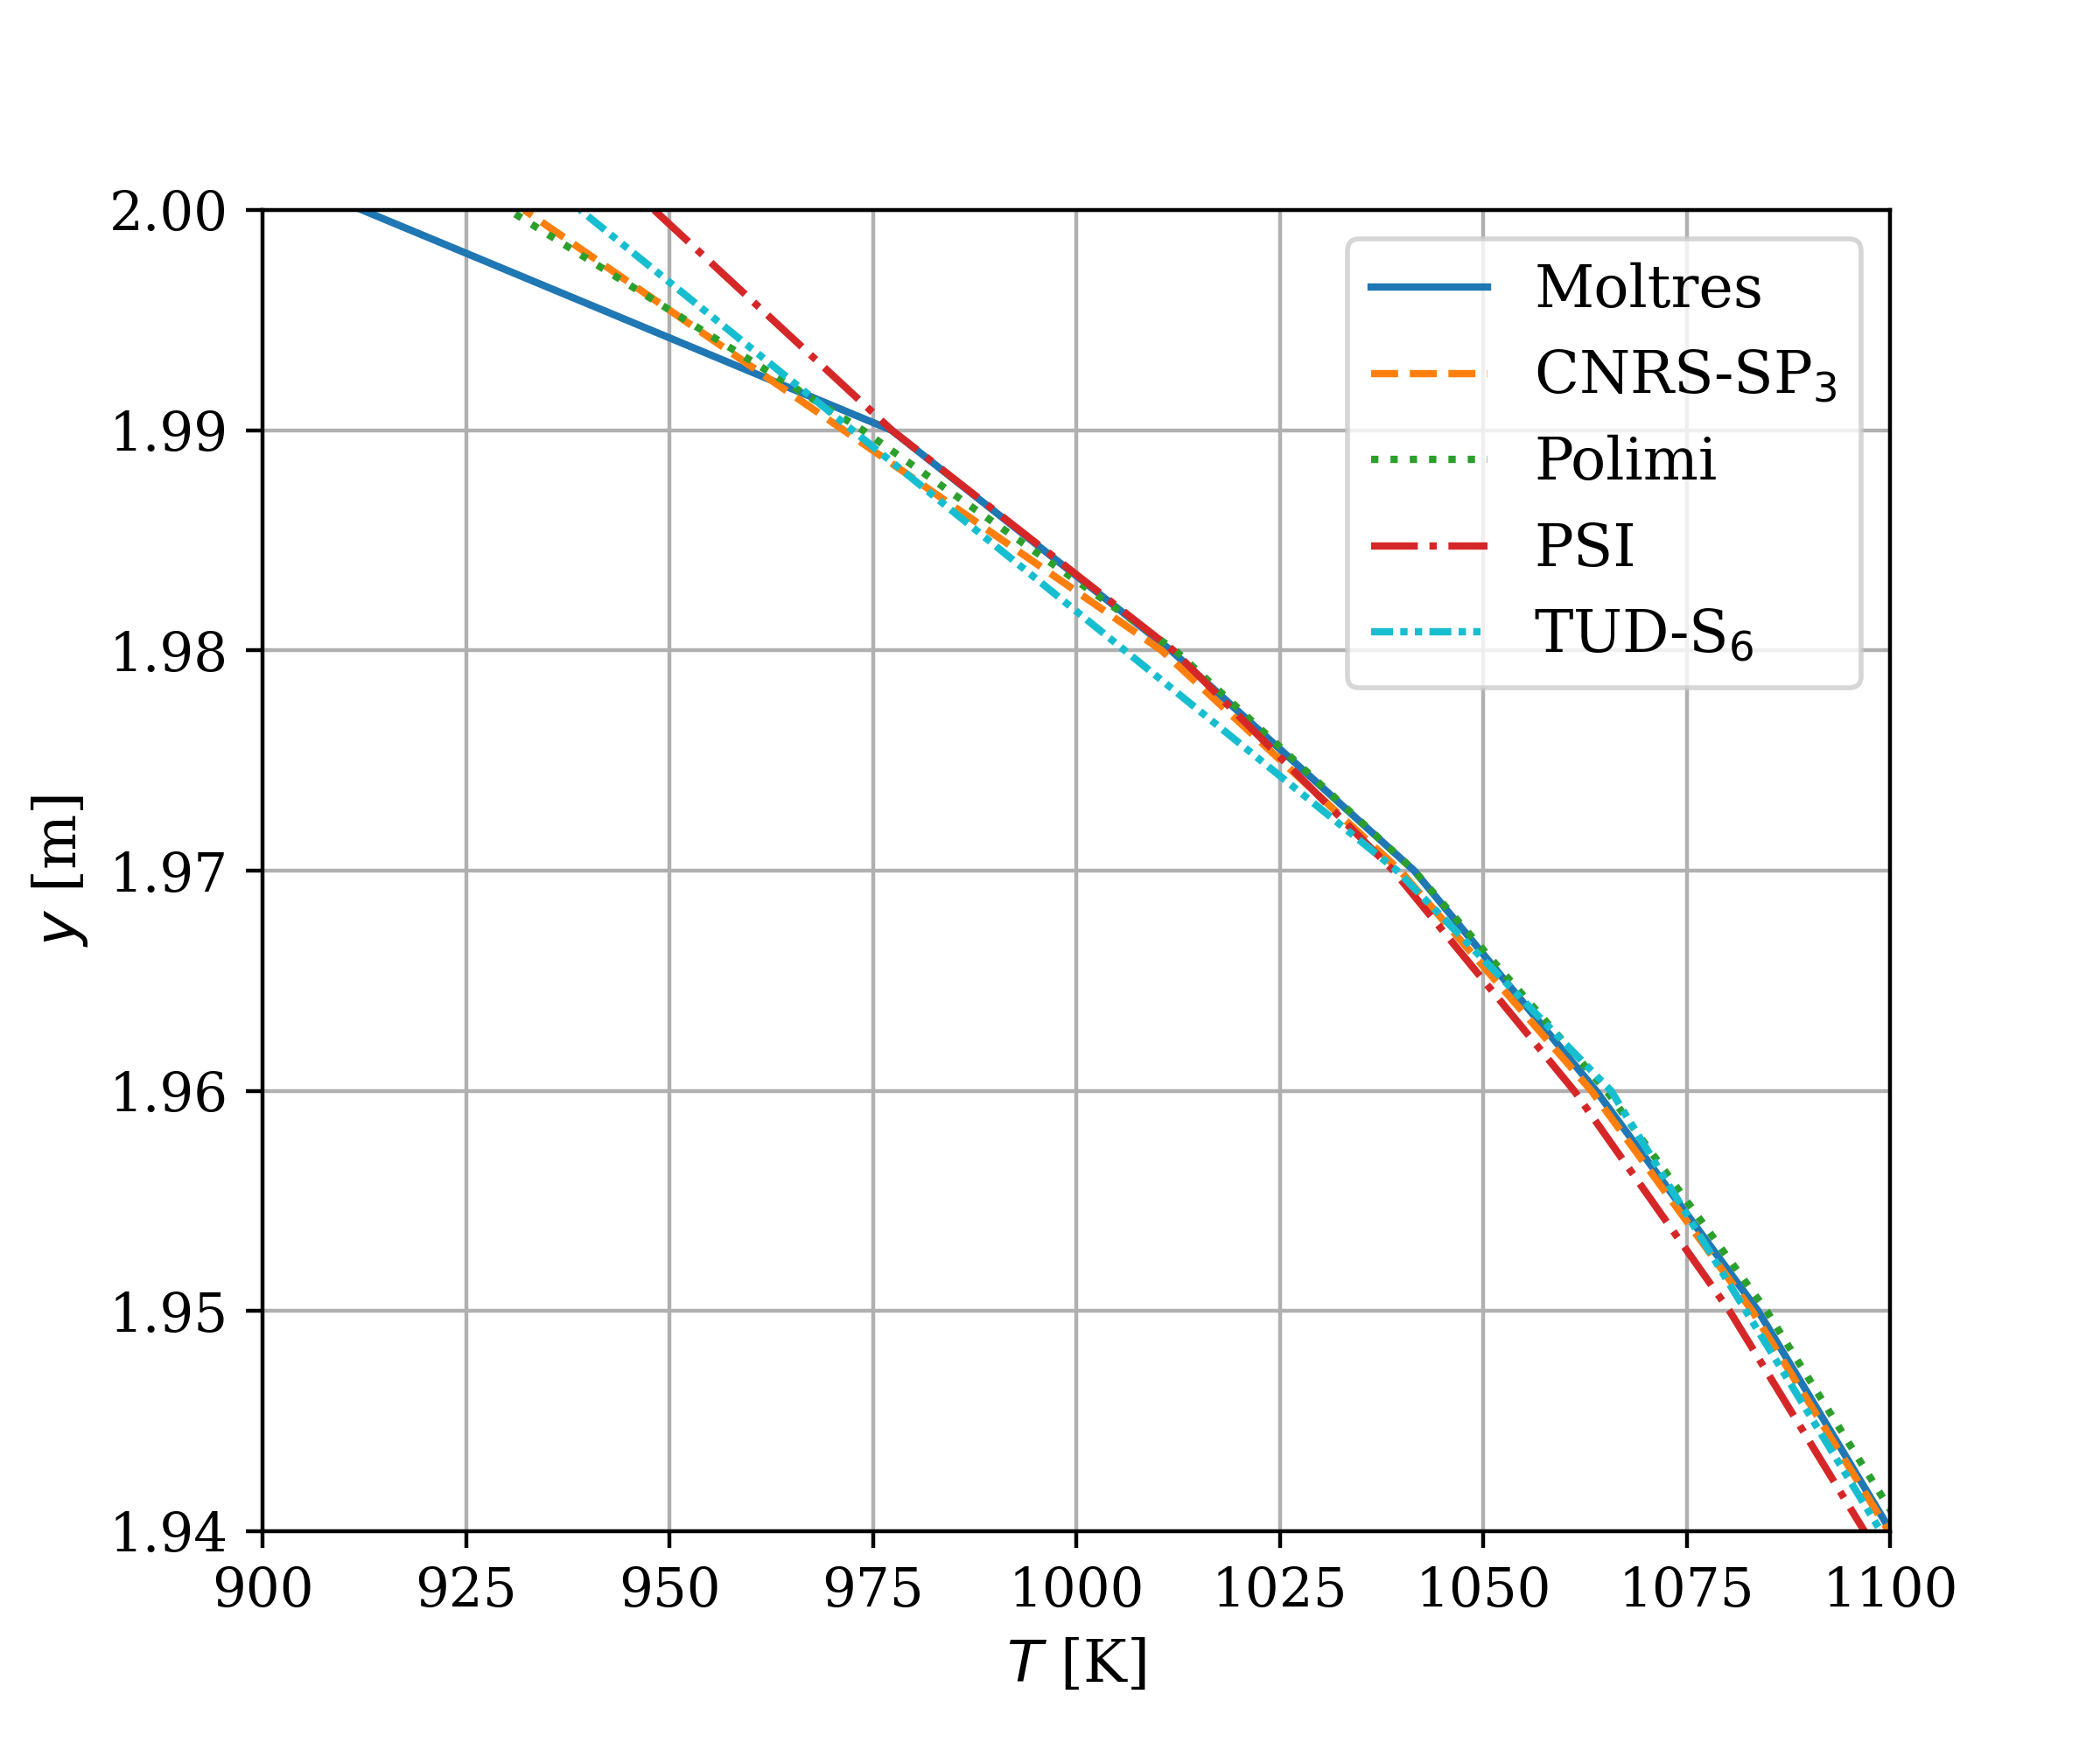
\includegraphics[width=.49\columnwidth]{0-3-temp-plot-zoom}
	\caption{Step 0.3 \textemdash\ Temperature distribution along BB' for y = 1.94 m to
	y = 2.00 m.}
	\label{fig:0.3-zoom}
\end{figure}

Lastly, we observe in table \ref{table:rho} that the reactivity $\rho$ value of
465.6 pcm from Moltres falls well within the range of $\rho$ values from the
benchmark, which range from 353.7 pcm up to 578.1 pcm. Given that Moltres 
adopts the neutron diffusion model, our $\rho$ value agrees closest to the
results from the software packages which also adopt the neutron diffusion model
or theoretically-equivalent models such as the $SP_1$ and $S_2$ neutron
transport models, namely CNRS-$SP_1$, PoliMi, PSI, and TUD-$S_2$.

\begin{table}[htb]
    \caption{Reactivity $\rho$ and change in reactivity
    $\left(\rho_a - \rho_b\right)$ values from Steps 0.2, 1.1,
    1.2, and 1.3. All units are in pcm.}
    \centering
    \small
    \setlength\tabcolsep{2pt}
    \begin{tabular}{l S S S S}
        \toprule
        \multirow{2}{*}{\textbf{Software}} & {\textbf{Step 0.2}} &
        {\textbf{Step 1.1}} & {\textbf{Step 1.2}} & {\textbf{Step 1.3}} \\
        & {$\rho_{s_{0.2}}$}
        & {$\rho_{s_{1.1}} - \rho_{s_{0.2}}$}
        & {$\rho_{s_{1.2}} - \rho_{s_{1.1}}$}
        & {$\rho_{s_{1.3}} - \rho_{s_{0.2}}$} \\
        \midrule
        Moltres     & 465.6 & -62.7 & -1142.2 & -1207.7 \\
        CNRS-$SP_1$ & 411.3 & -62.5 & -1152.0 & -1220.5 \\
        CNRS-$SP_3$ & 353.7 & -62.6 & -1152.7 & -1220.7 \\
        PoliMi      & 421.2 & -62.0 & -1161.0 & -1227.0 \\
        PSI         & 411.7 & -63.0 & -1154.8 & -1219.6 \\
        TUD-$S_2$   & 482.6 & -62.0 & -1145.2 & -1208.5 \\
        TUD-$S_6$   & 578.1 & -60.7 & -1122.0 & -1184.4 \\
        \bottomrule
    \end{tabular}
    \label{table:rho}
\end{table}

\FloatBarrier

\subsubsection{Phase 1 results \& discussion}

Table \ref{table:disc1} shows the discrepancy values from Moltres relative to
the average and \gls{SD} of the benchmark participants for Steps 1.1, 1.2, and
1.3 and the corresponding average discrepancy values from the benchmark
\cite{tiberga_results_2020}. The subsequent subsections discuss the results
for each benchmark step in Phase 1.
%
\begin{table}[htb]
	\caption{Discrepancy values from Moltres alongside the average and standard
	deviation of the discrepancy values of the benchmark participants for Phase
	1.}
	\centering
	\small
	\begin{tabular}{l l c S S S}
		\toprule
		\multirow{2}{*}{\textbf{Step}} & \multirow{2}{*}{\textbf{Observable}} & \multirow{2}{*}{\textbf{Centerline}} & {\multirow{2}{*}{\textbf{Moltres [\%]}}} & \multicolumn{2}{c}{\textbf{Benchmark [\%]}} \\
		& & & & {Average} & {SD} \\
		\midrule
		\multirow{2}{*}{1.1} &
		\multirow{2}{*}{$\sum_i \lambda_i C_i$} & AA' & 0.603 & 0.346 & 0.166
		\\
		& & BB' & 0.327 & 0.294 & 0.153 \\
		\midrule
		\multirow{4}{*}{1.2} &
		\multirow{2}{*}{$T$} & AA' & 0.076 & 0.095 & 0.015 \\
		& & BB' & 0.179 & 0.089 & 0.012 \\
		\cmidrule{2-6}
		& \multirow{2}{*}{\footnotesize $\Delta\left[\sum^6_g \Sigma_{f,g} \phi_g(\vec{r})
		\right]_{s_{1.2}-s_{0.2}}$} & AA' & 1.110 & 1.576 & 0.564 \\
		& & BB' & 1.089 & 1.133 & 0.392 \\
		\midrule
		\multirow{7}{*}{1.3} &
		{$u_x$} & AA' & 0.123 & 0.691 & 0.566 \\
		\cmidrule{2-6}
		& \multirow{2}{*}{$u_y$} & AA' & 0.237 & 0.329 & 0.131 \\
		& & BB' & 0.238 & 0.356 & 0.217 \\
		\cmidrule{2-6}
		& \multirow{2}{*}{$T$} & AA' & 0.064 & 0.057 & 0.023 \\
		& & BB' & 0.070 & 0.080 & 0.024 \\
		\cmidrule{2-6}
		& \multirow{2}{*}{$\sum_i \lambda_i C_i$} & AA' & 1.043 & 0.460 & 0.190
		\\
		& & BB' & 0.462 & 1.194 & 0.178 \\
		\bottomrule
	\end{tabular}
	\label{table:disc1}
\end{table}

\paragraph{Step 1.1: Circulating fuel}

Figure \ref{fig:1.1} shows good qualitative agreement in the delayed neutron
source distribution along BB' among Moltres and the benchmark participants.
From Table \ref{table:disc1}, Moltres reports discrepancies of 0.603\% and
0.327\% along the centerlines AA' and BB', respectively. Both values are
within two and one \gls{SD}, respectively, of the average discrepancies of the
benchmark participants (0.346\% and 0.294\%).
In Table \ref{table:rho}, we observe that the change in
$\rho$ relative to Step 0.2 is $-62.7$ pcm for Moltres, and this value is
consistent with the $-63.0$ to $-62.0$ pcm range that most of the benchmark
participants' values fall in.
%
\begin{figure}[htb]
	\centering
    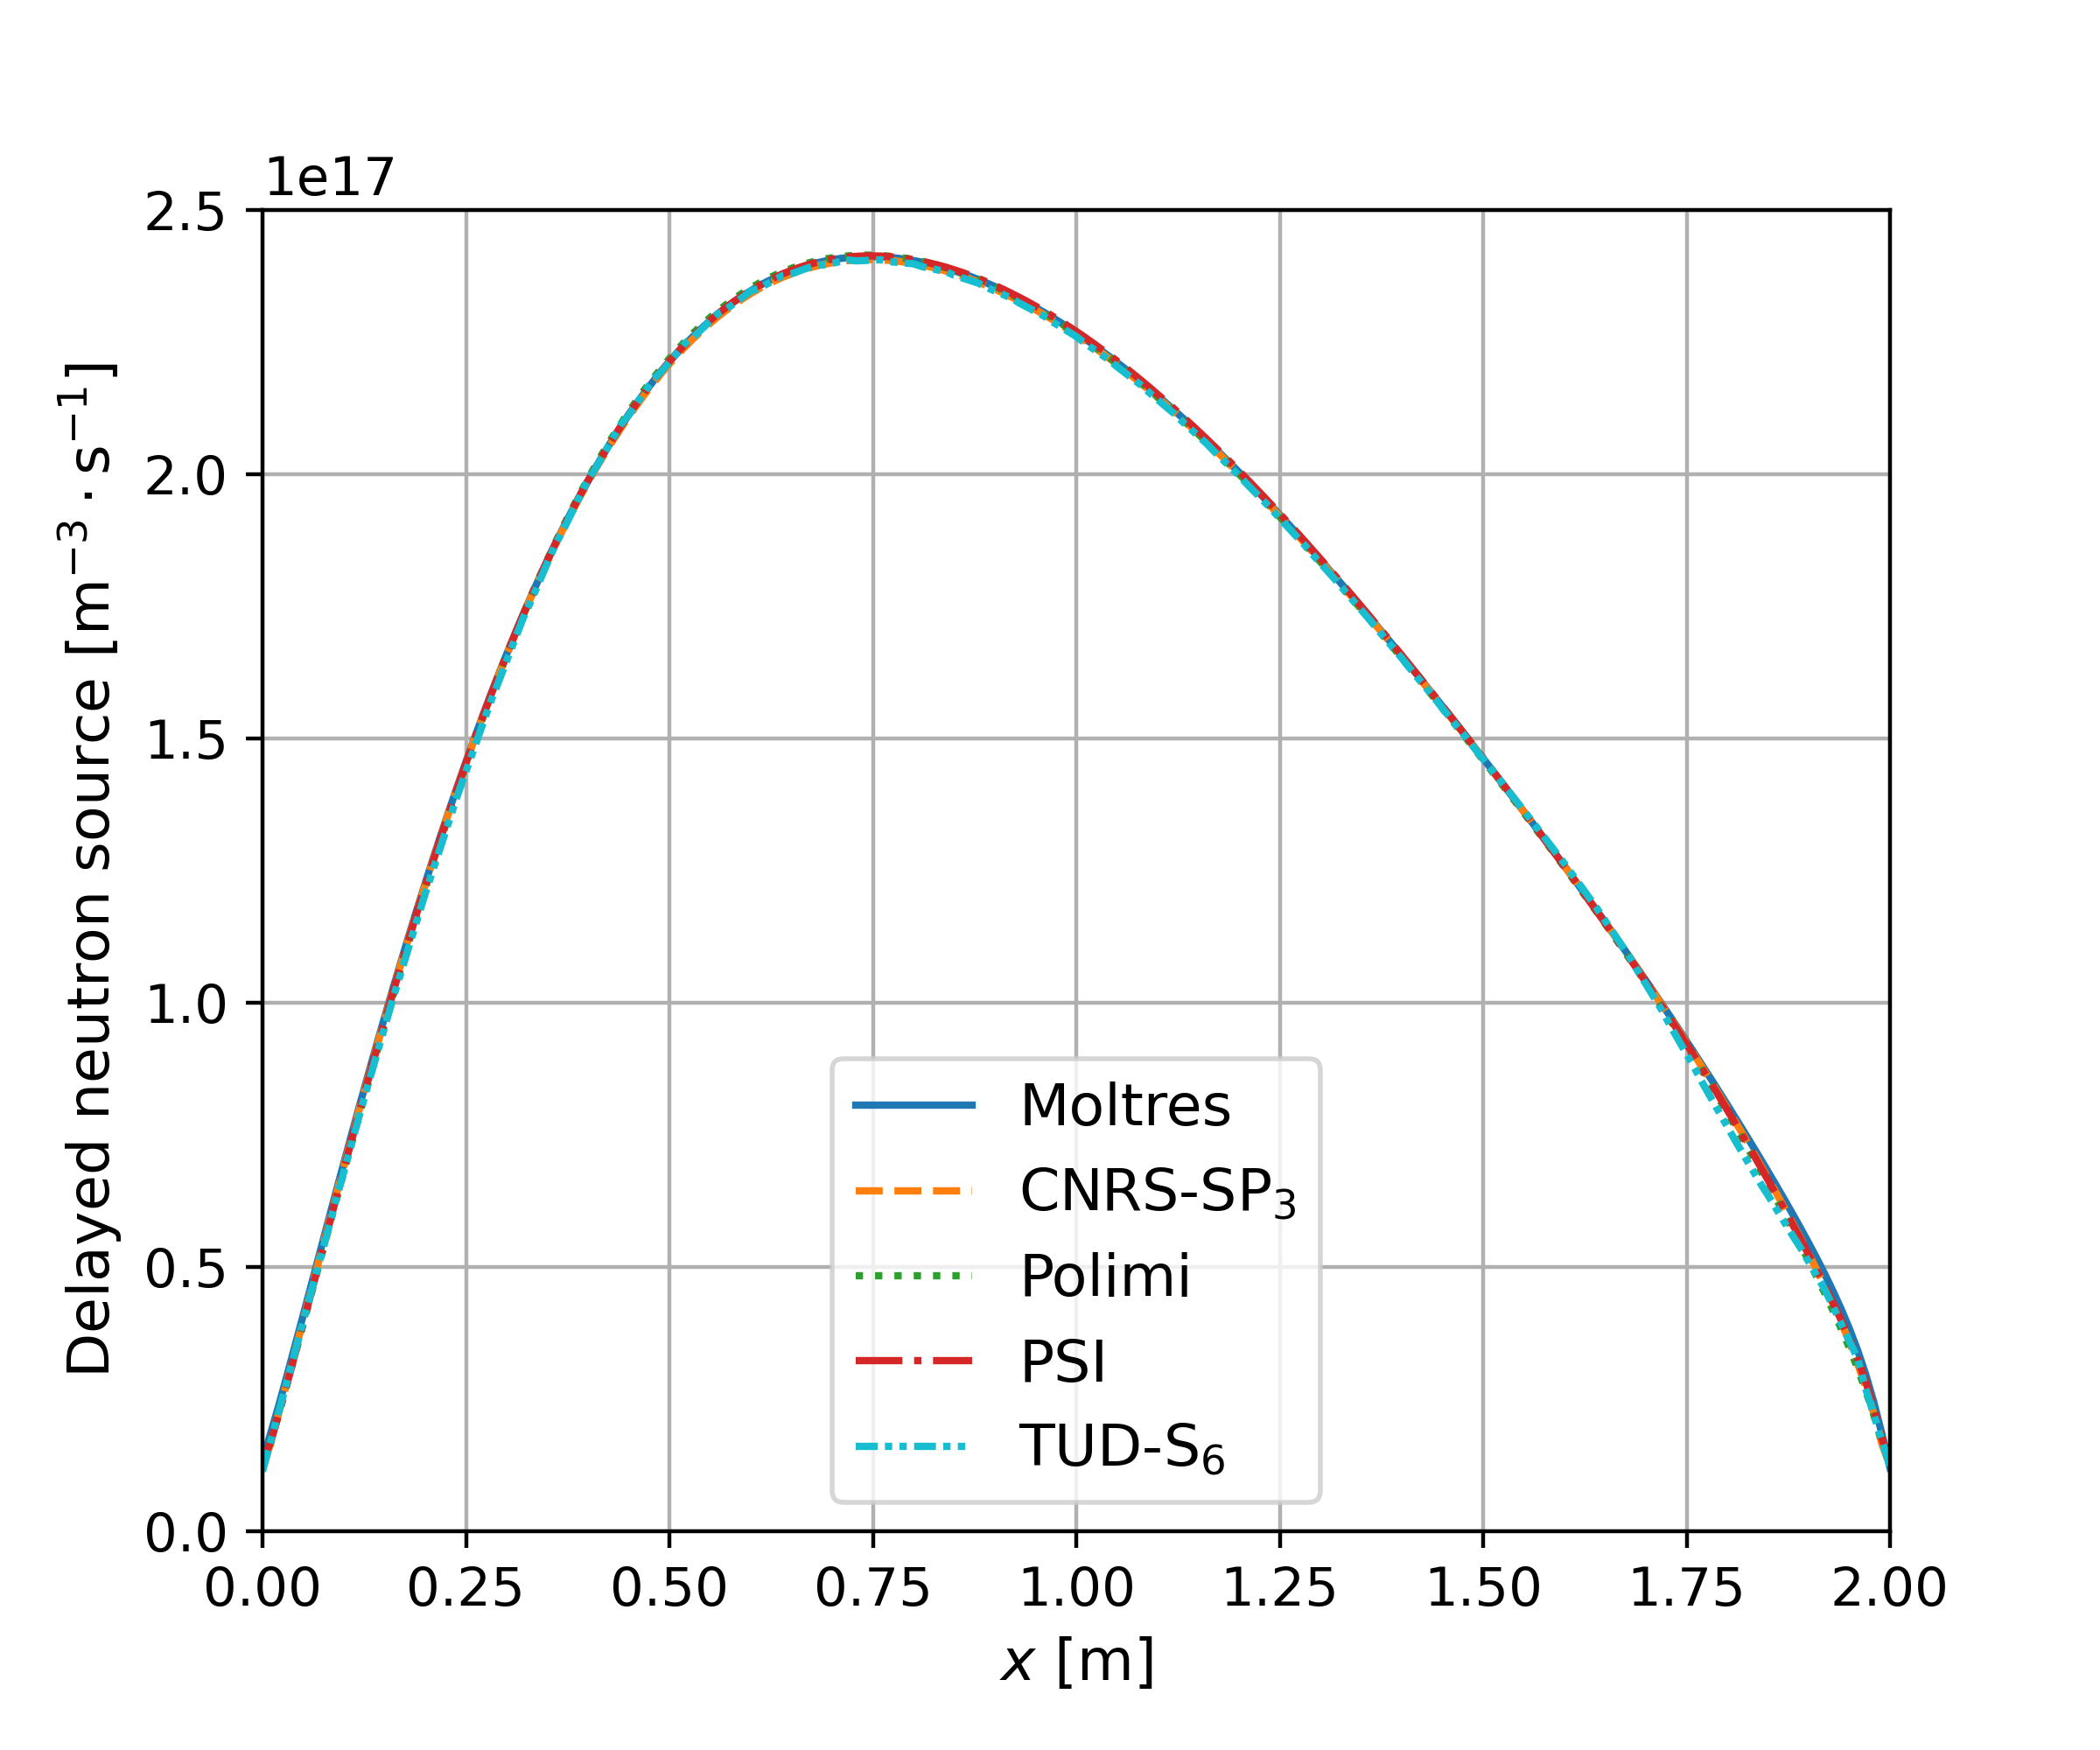
\includegraphics[width=.49\columnwidth]{1-1-dnp-x-plot}
    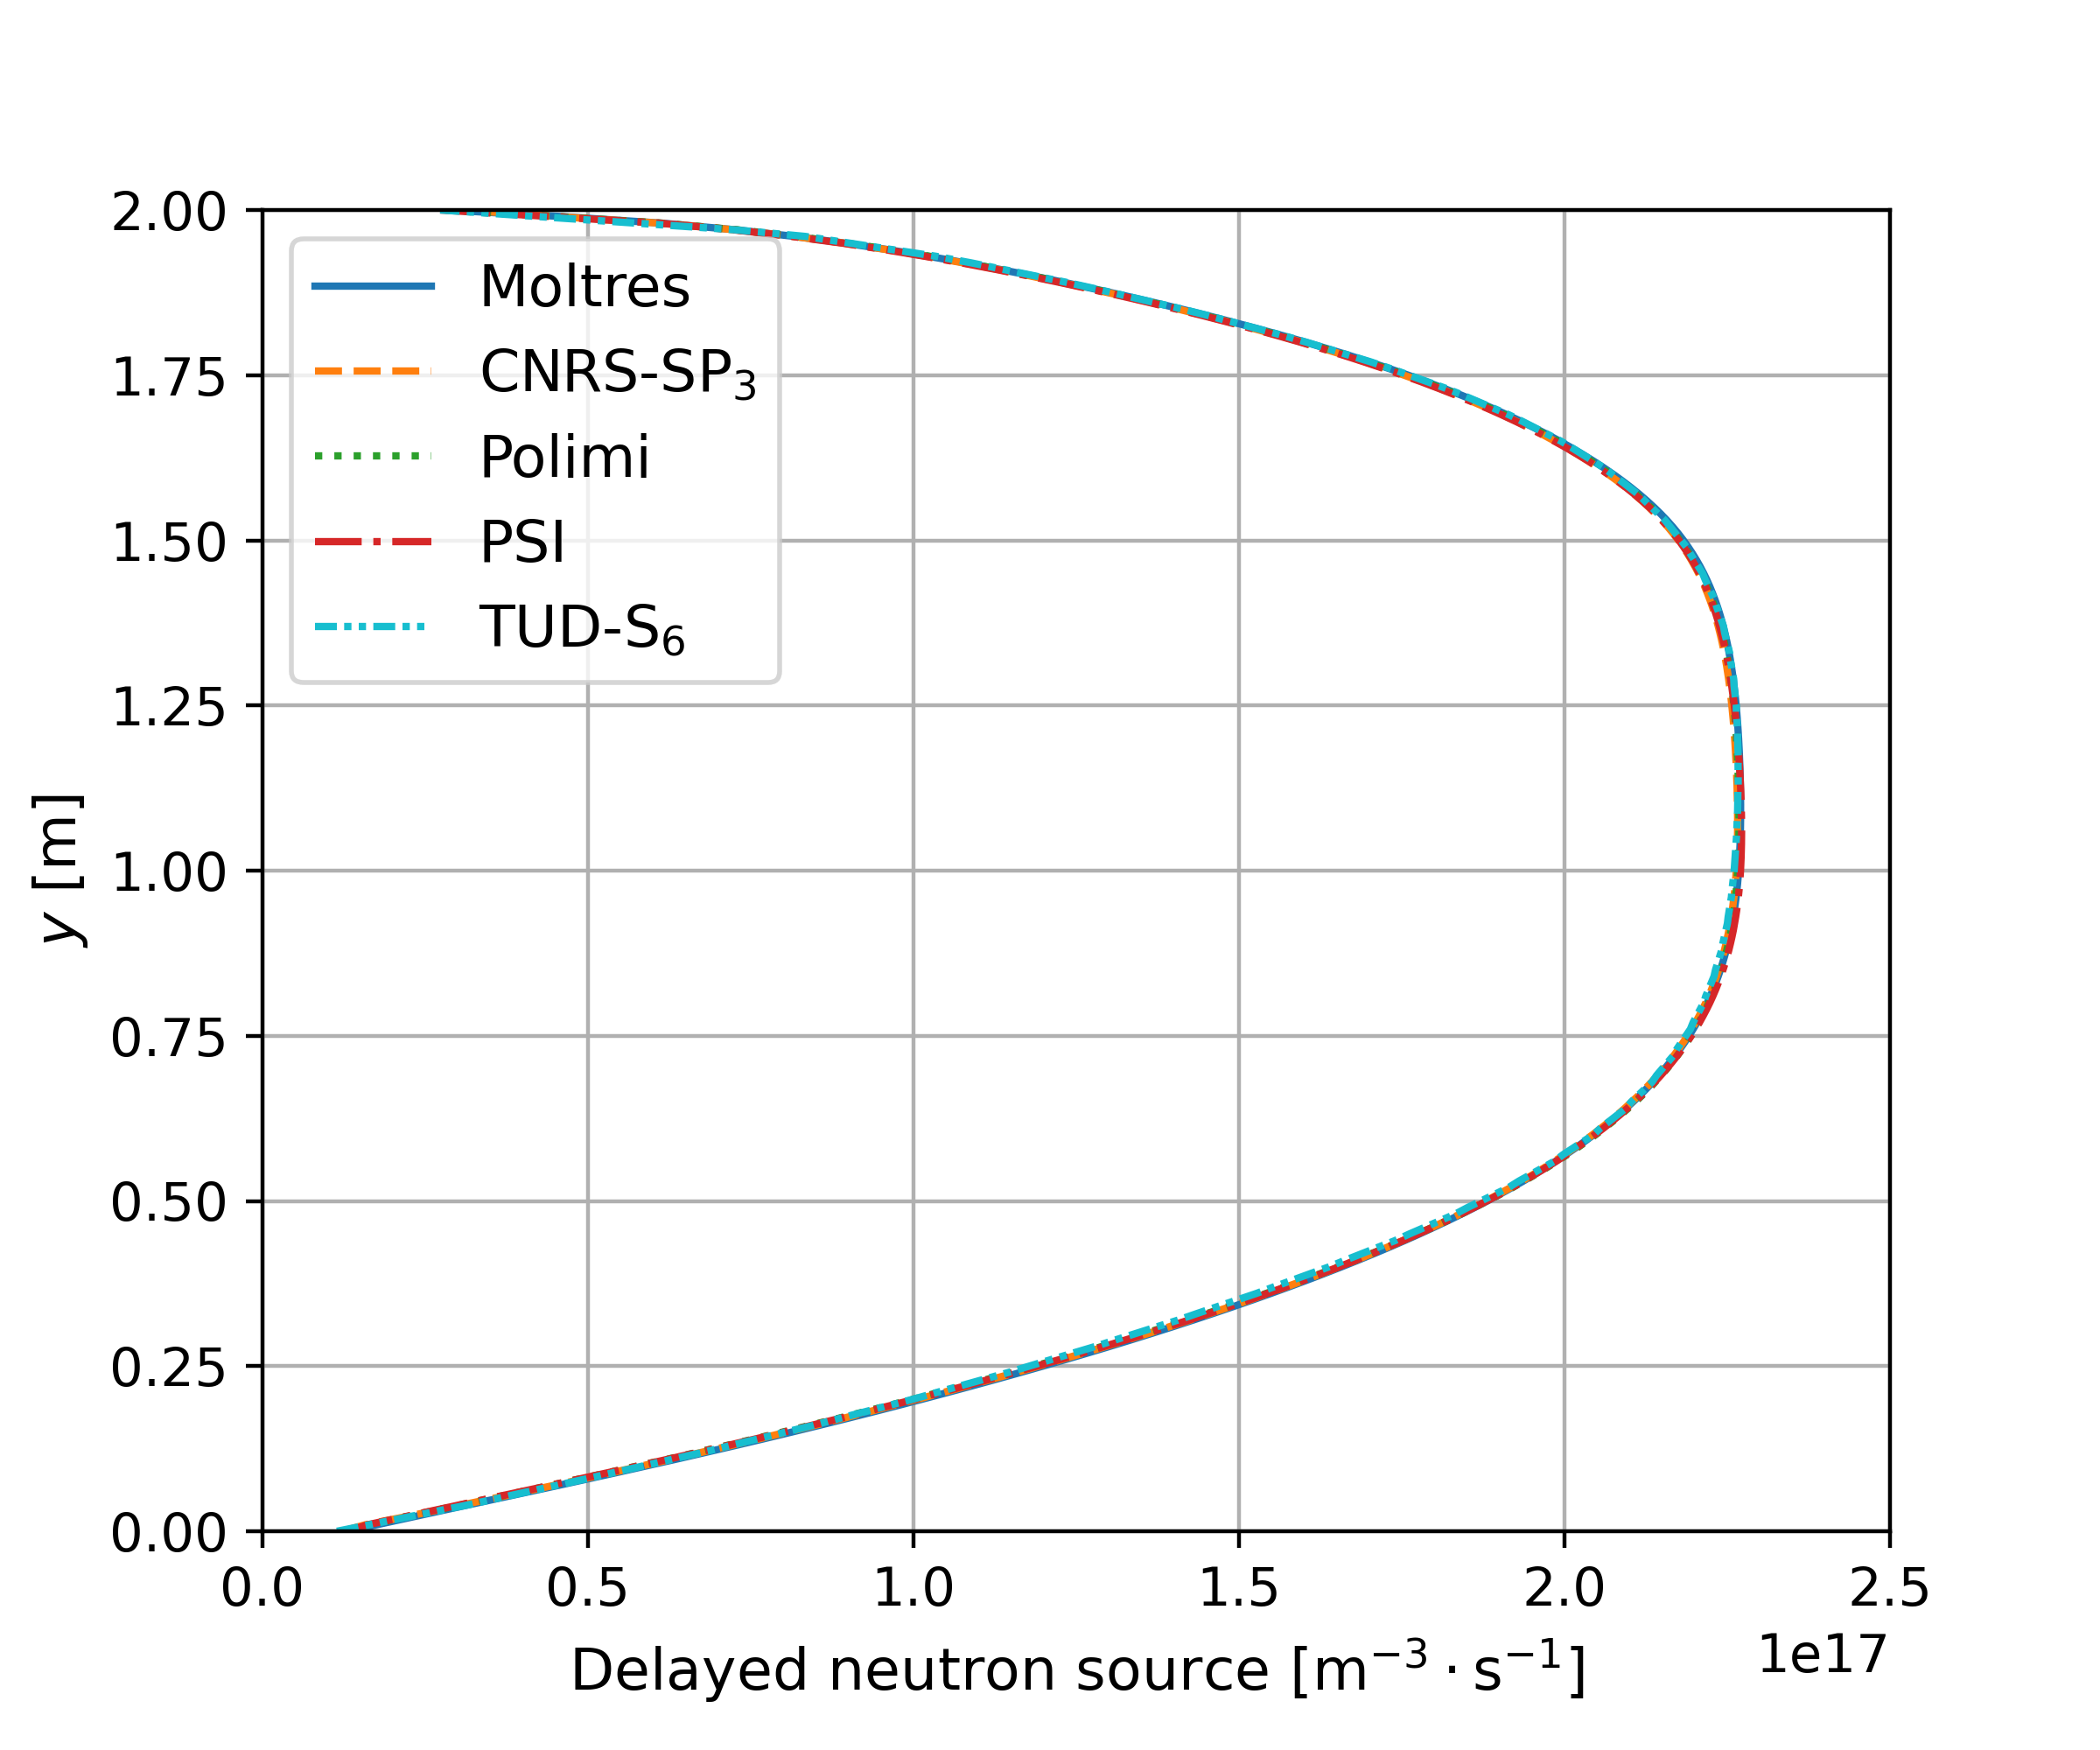
\includegraphics[width=.49\columnwidth]{1-1-dnp-y-plot}
	\caption{Step 1.1 \textemdash\ Delayed neutron source along AA' (top) and BB'
	(bottom).}
	\label{fig:1.1}
\end{figure}
%
\begin{figure}[htb]
	\centering
	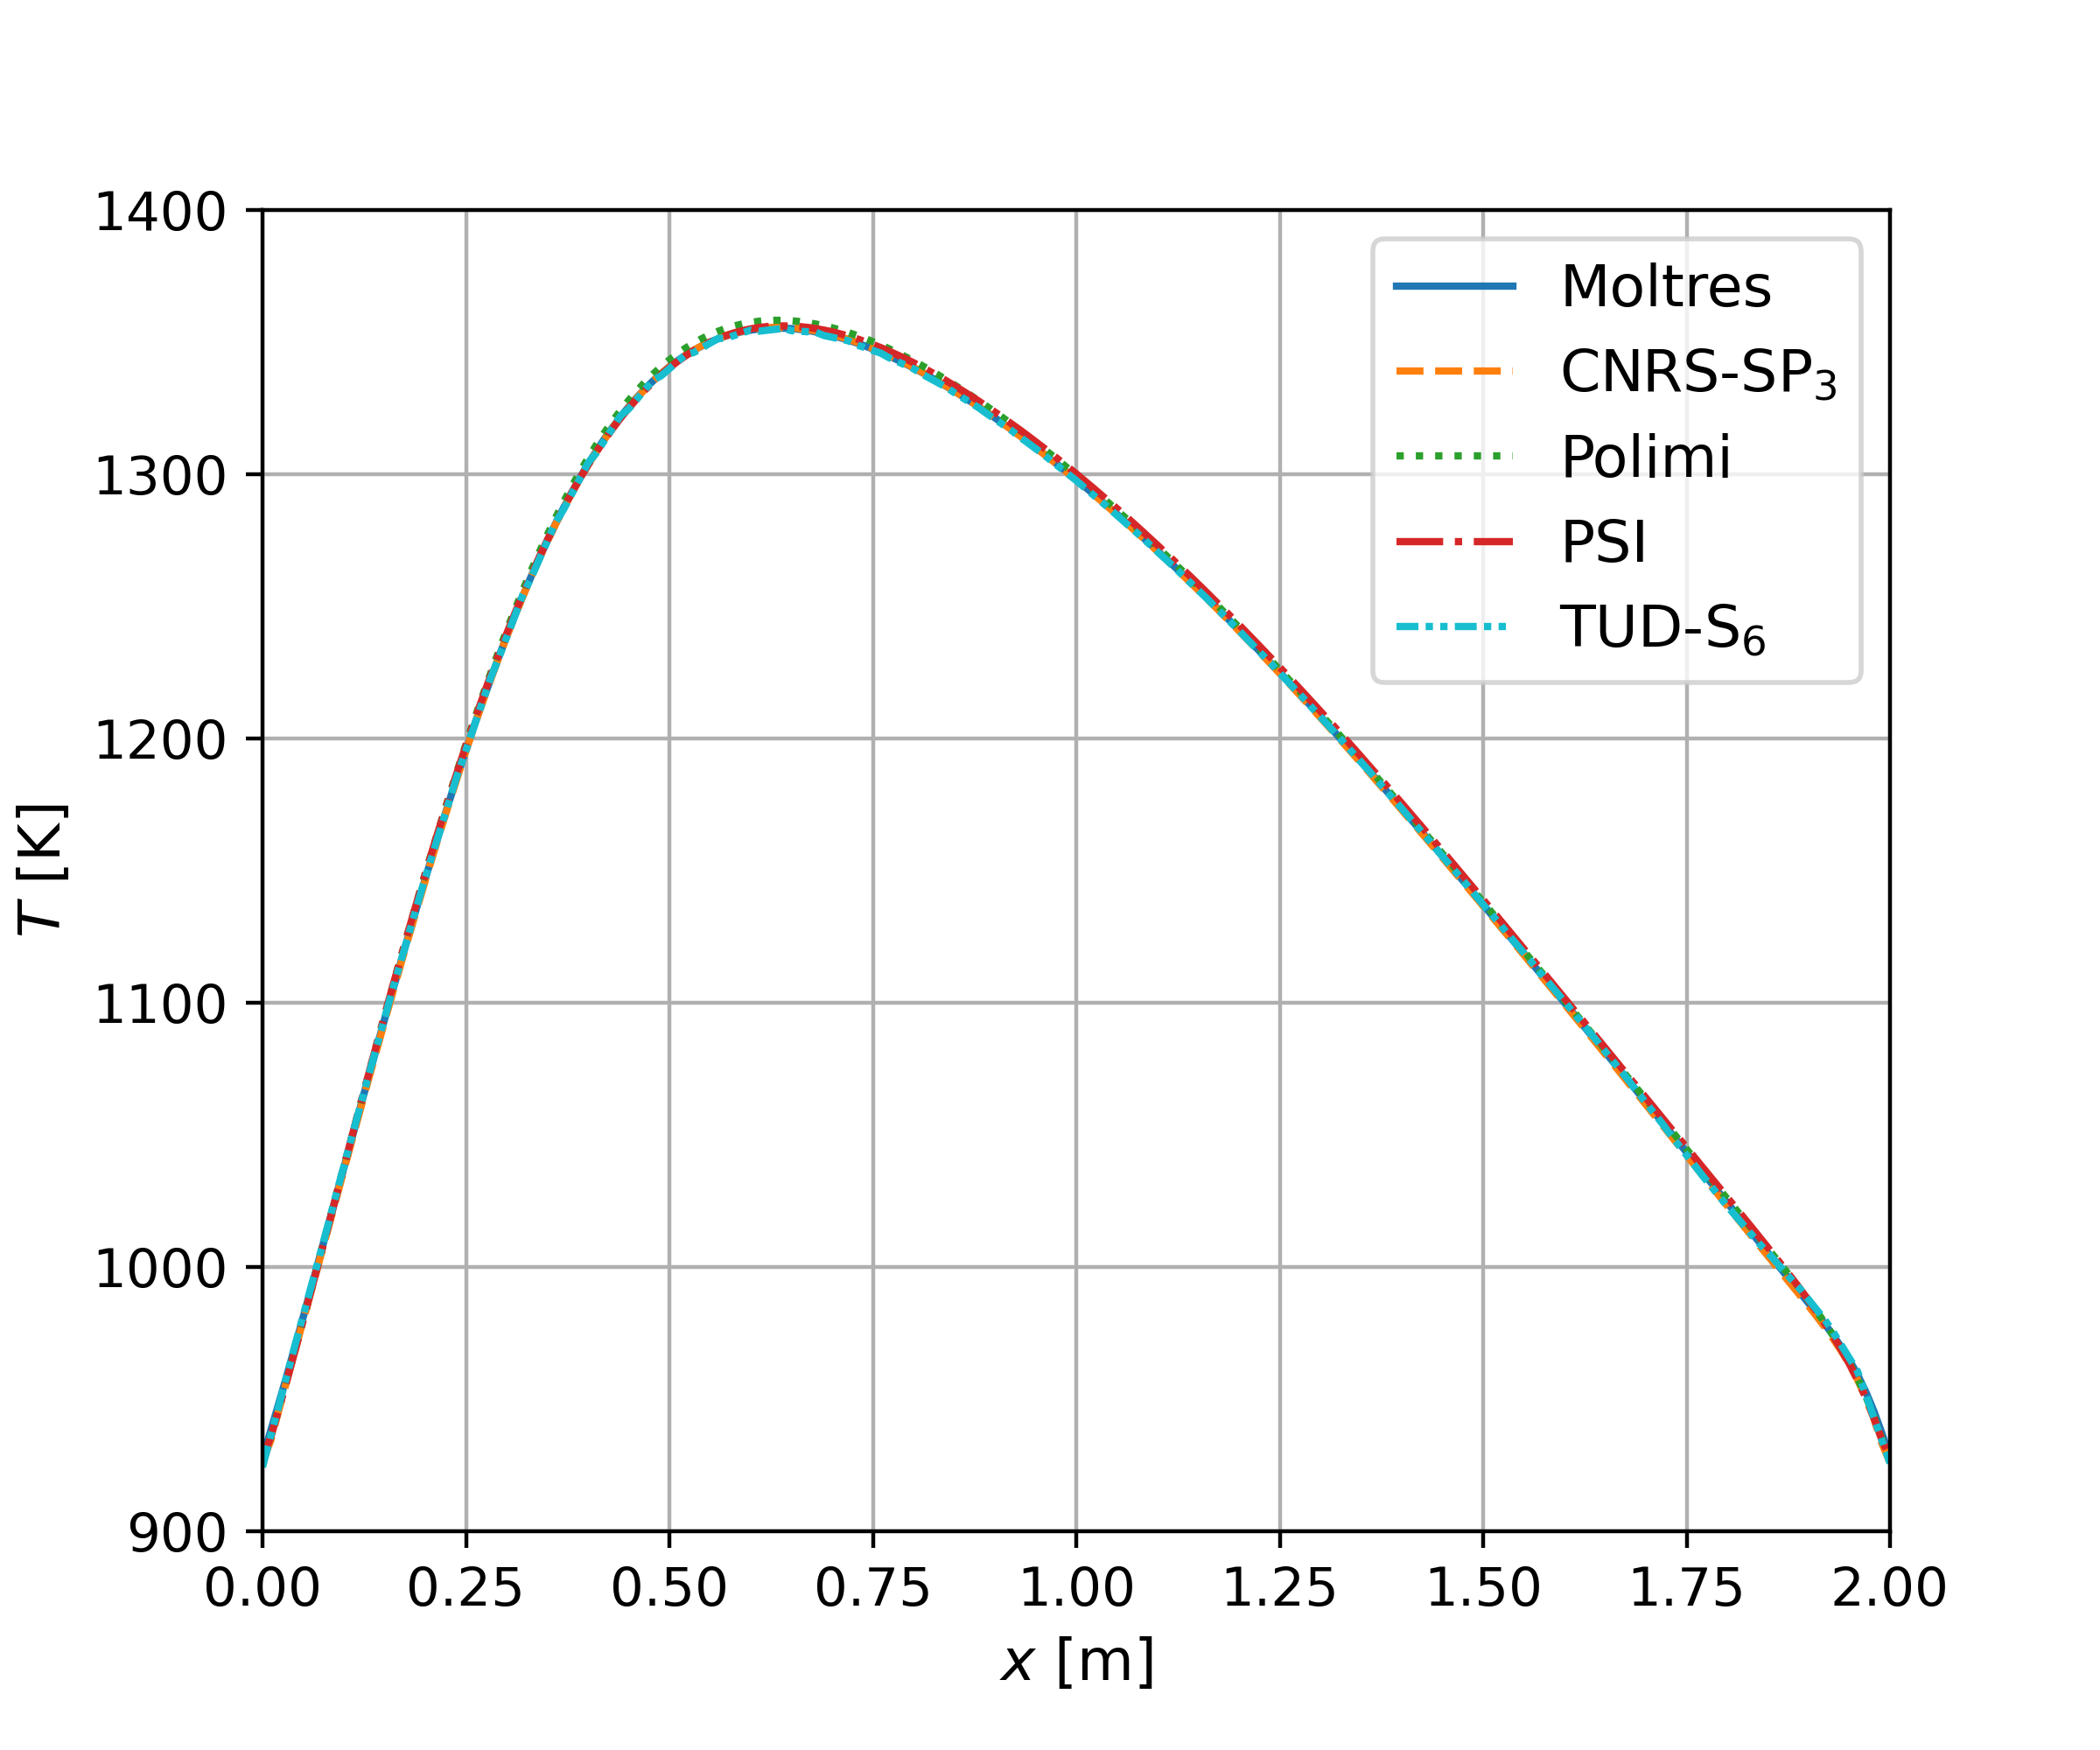
\includegraphics[width=.49\columnwidth]{1-2-temp-plot}
	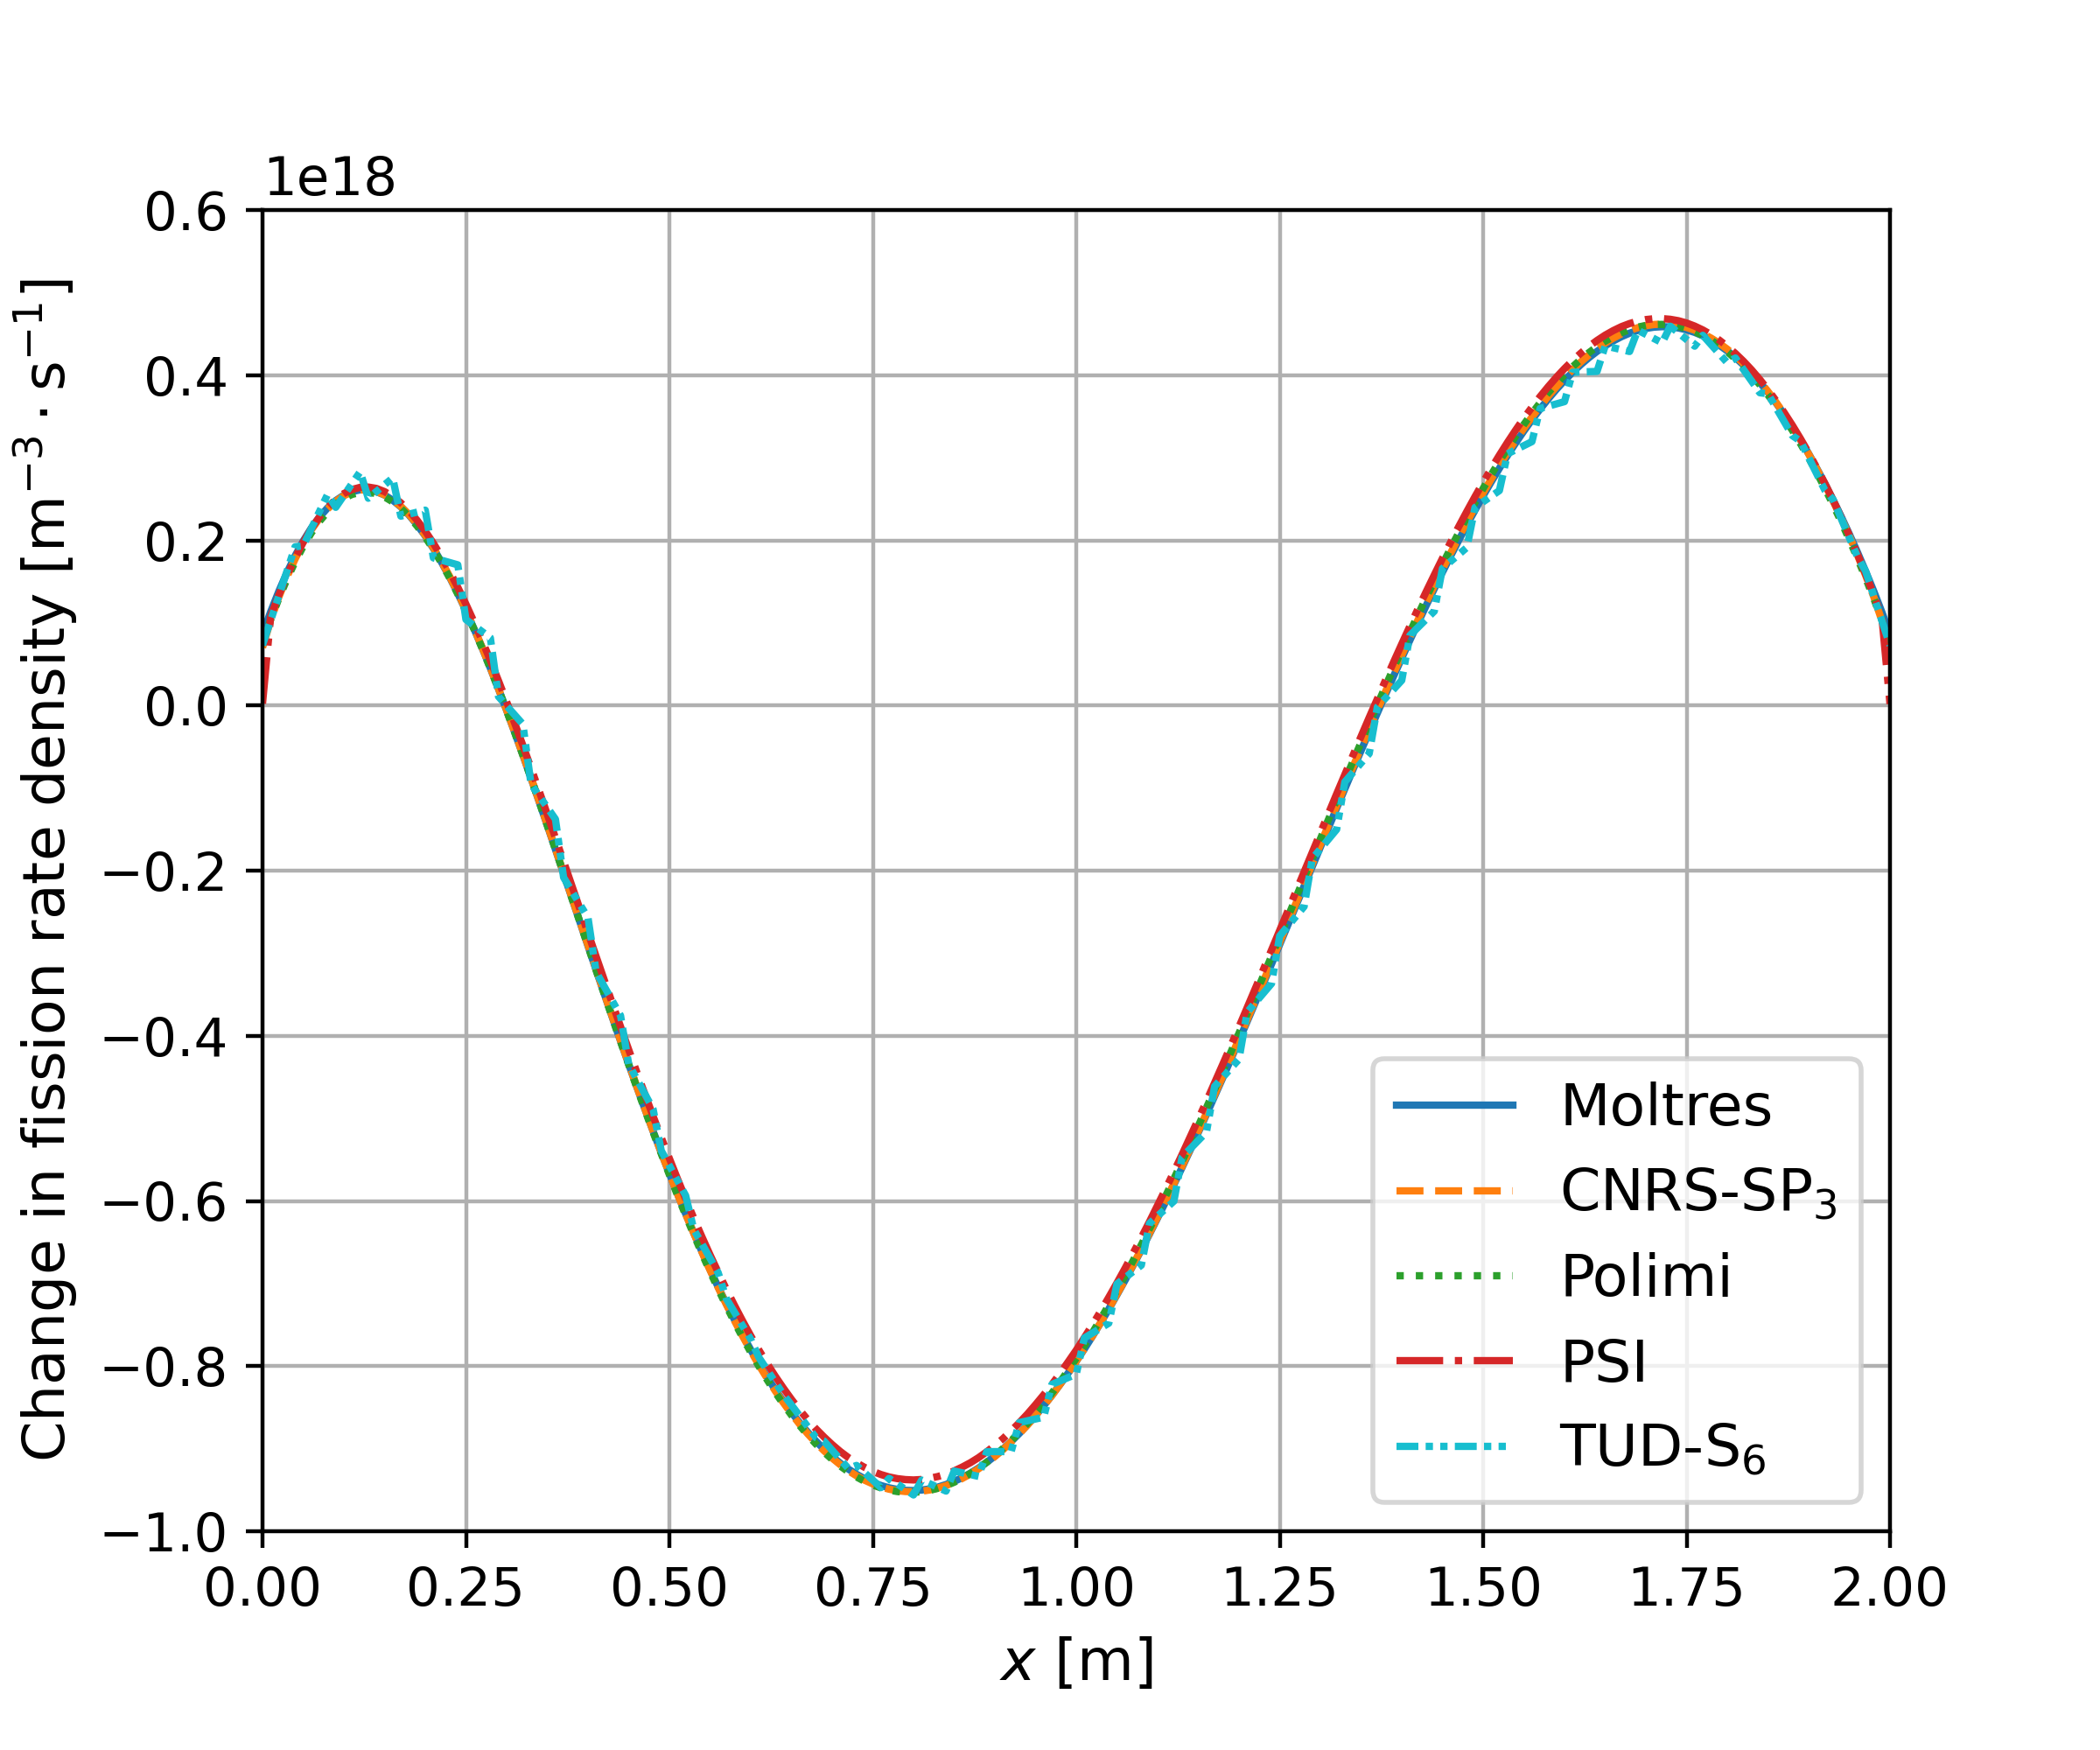
\includegraphics[width=.49\columnwidth]{1-2-fiss-plot}
	\caption{Step 1.2 \textemdash\ Temperature distribution and change in fission rate
	density along AA'.}
	\label{fig:1.2}
\end{figure}

\FloatBarrier

\paragraph{Step 1.2: Power coupling}

Figure \ref{fig:1.2} shows the temperature distribution and the change in
fission rate density along AA' from Step 1.2. Similar to Step 0.3, the
temperature distribution from Moltres agrees closest with CNRS-$SP_3$ and
TUD-$S_2$. Table \ref{table:disc1} reports the same trends we observed in Phase
0; the average discrepancy in temperature along BB' from Moltres for Step 1.2
is marginally higher than the benchmark, while the average discrepancy in the
fission rate density is within one \gls{SD} range to the benchmark average.
From Table \ref{table:rho}, Moltres also reports a change in $\rho$
relative to Step 1.1 of $-1142.2$ pcm, which
falls within the range of reported benchmark participants' values.

\paragraph{Step 1.3: Buoyancy}

Figure \ref{fig:1.3} shows the vertical velocity component, temperature, and
delayed neutron source distributions along AA'.
Moltres reproduces the correct trend in all three physical
observables. Step 1.3 has a relatively slower buoyancy-driven flow profile with
no forced flow from the top boundary. Consequently, there are no temperature
deviations near the top boundary, and we observe in Table \ref{table:disc1} that
the average discrepancy value of 0.070\% for the temperature distribution along
BB' is in much closer agreement to the benchmark value of 0.080\% compared to
the corresponding temperature discrepancy values for Step 0.3 and 1.2.

Table \ref{table:rho} shows that the change in $\rho$ from
Moltres (-1207.7 pcm) falls within the range of reported benchmark values and
matches the software from TUD-$S_2$ (-1208.5 pcm) the closest. This observation is likely
due to the similar solvers (diffusion and $S_2$ neutronics models) and
methods of solution (finite element method on uniform meshes) employed by our
respective software.
%
\begin{figure}[htb]
	\centering
	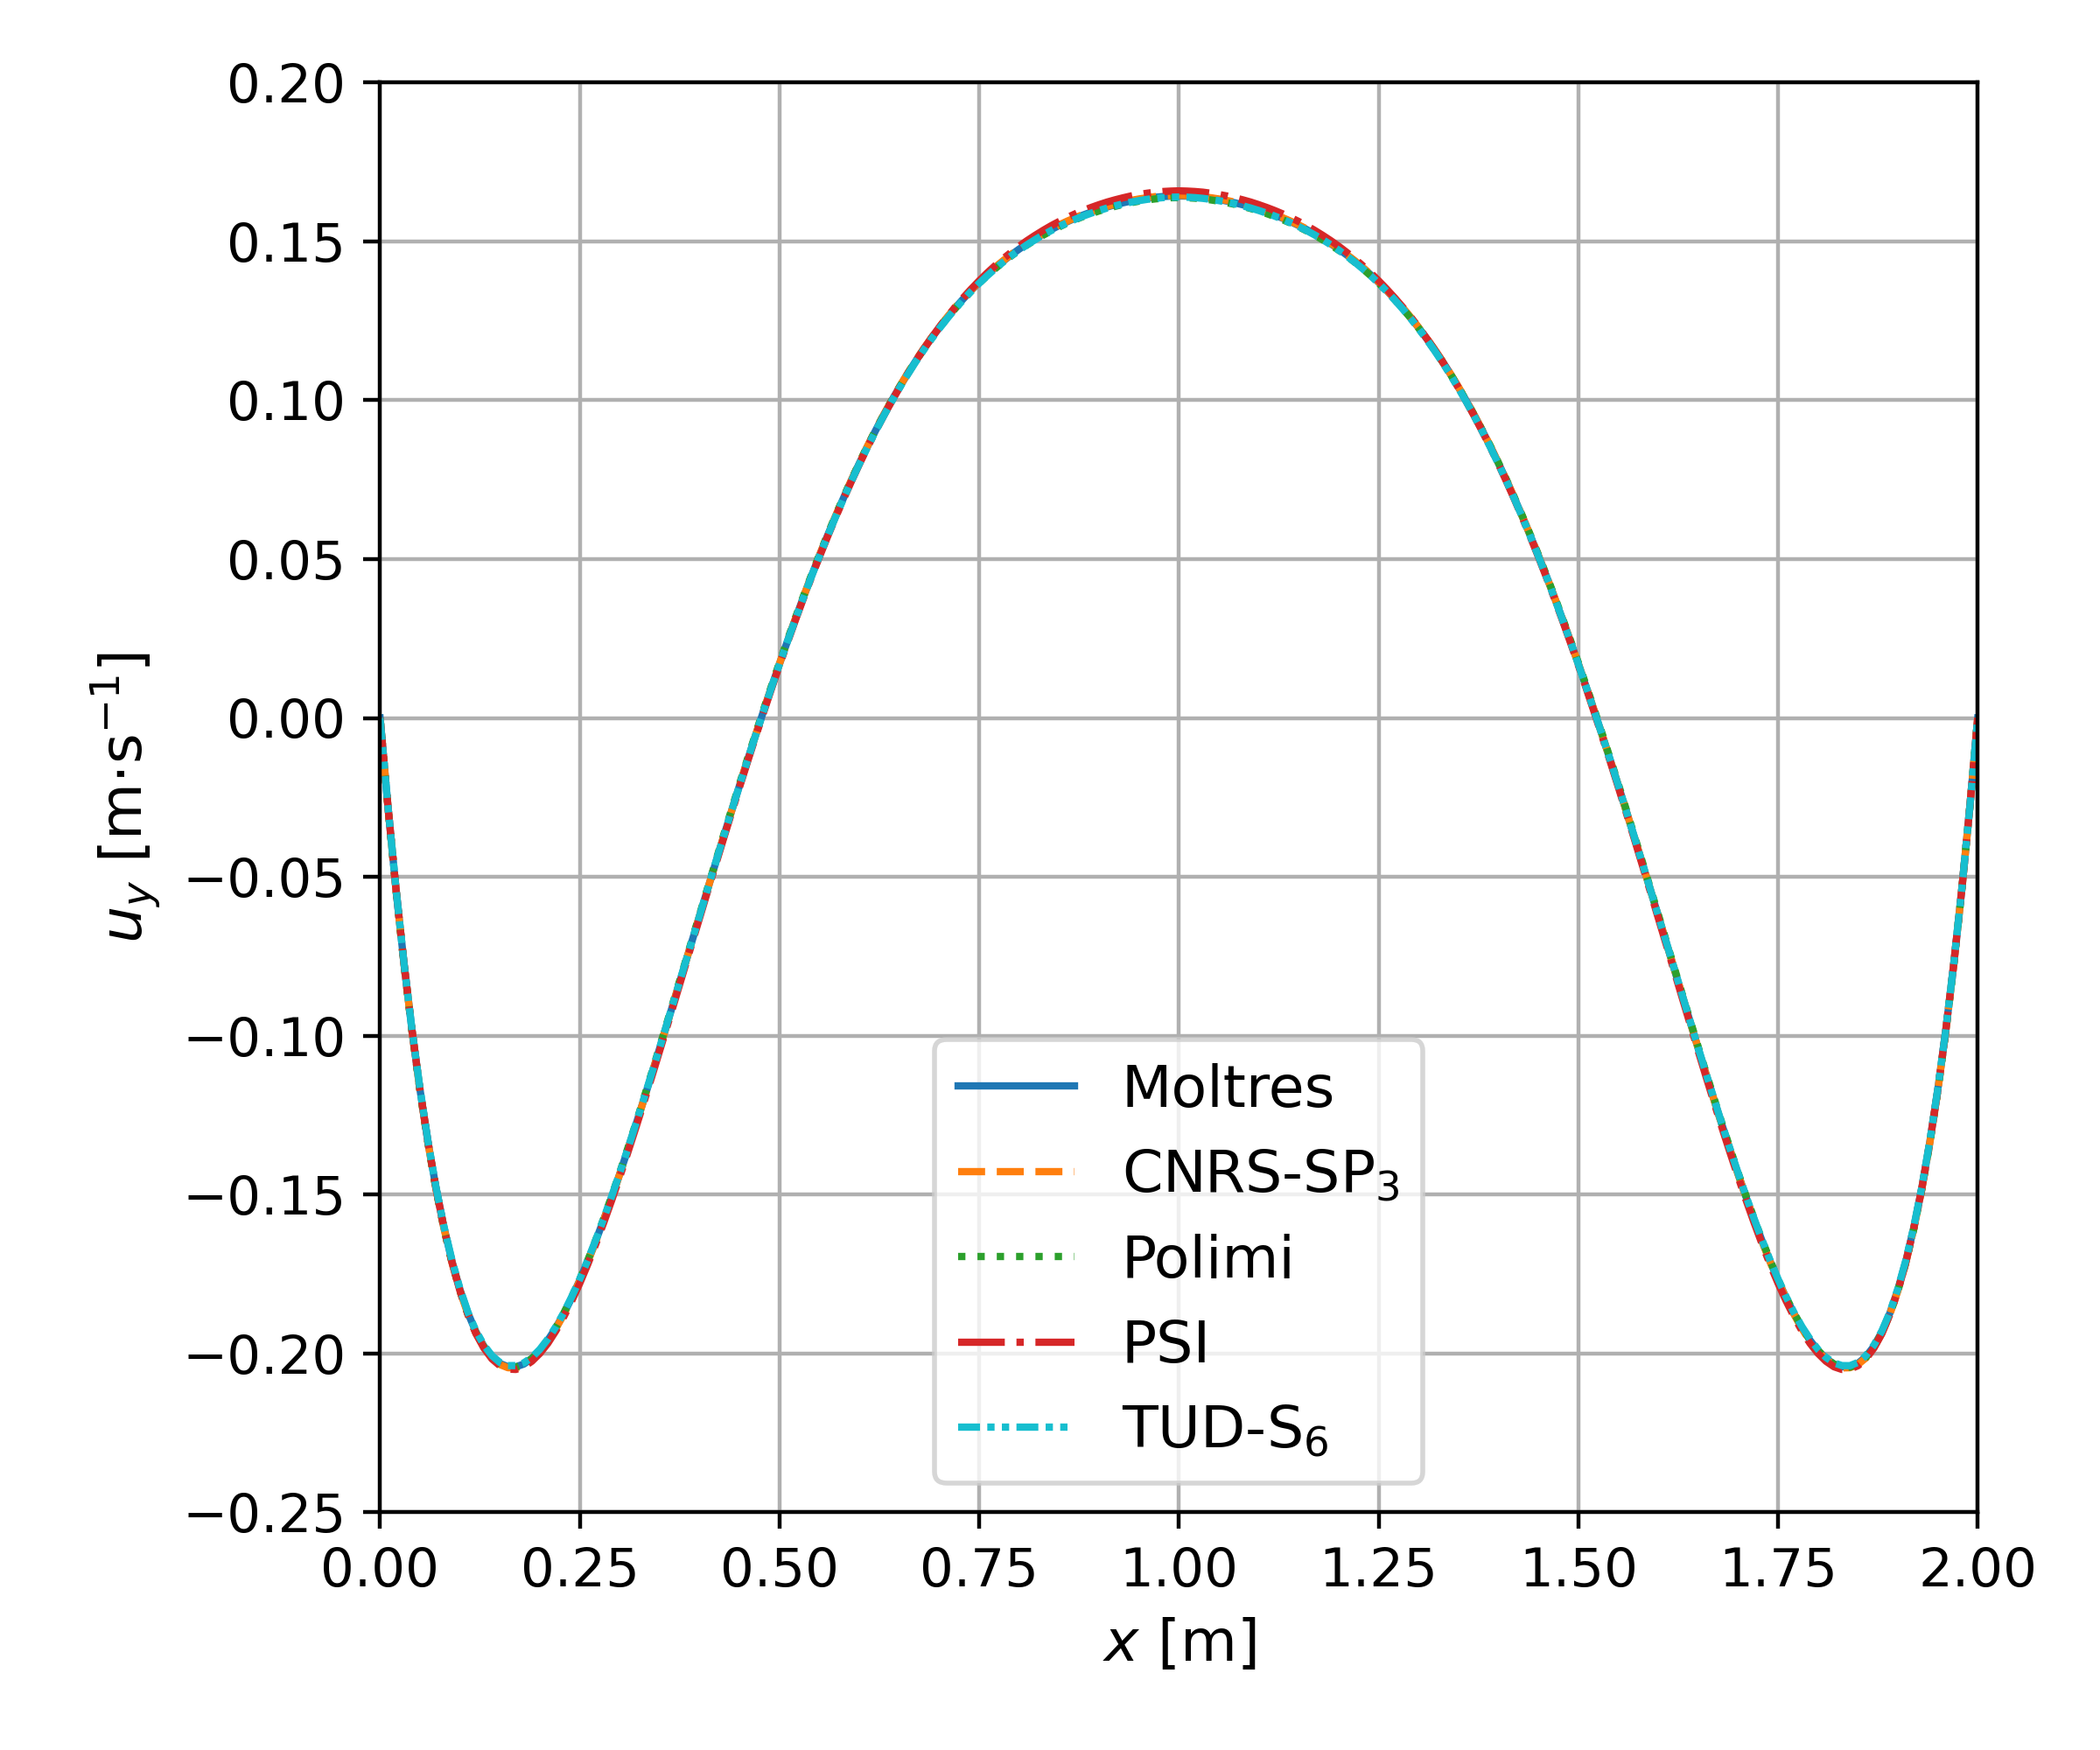
\includegraphics[width=.49\columnwidth]{1-3-vel-plot}
	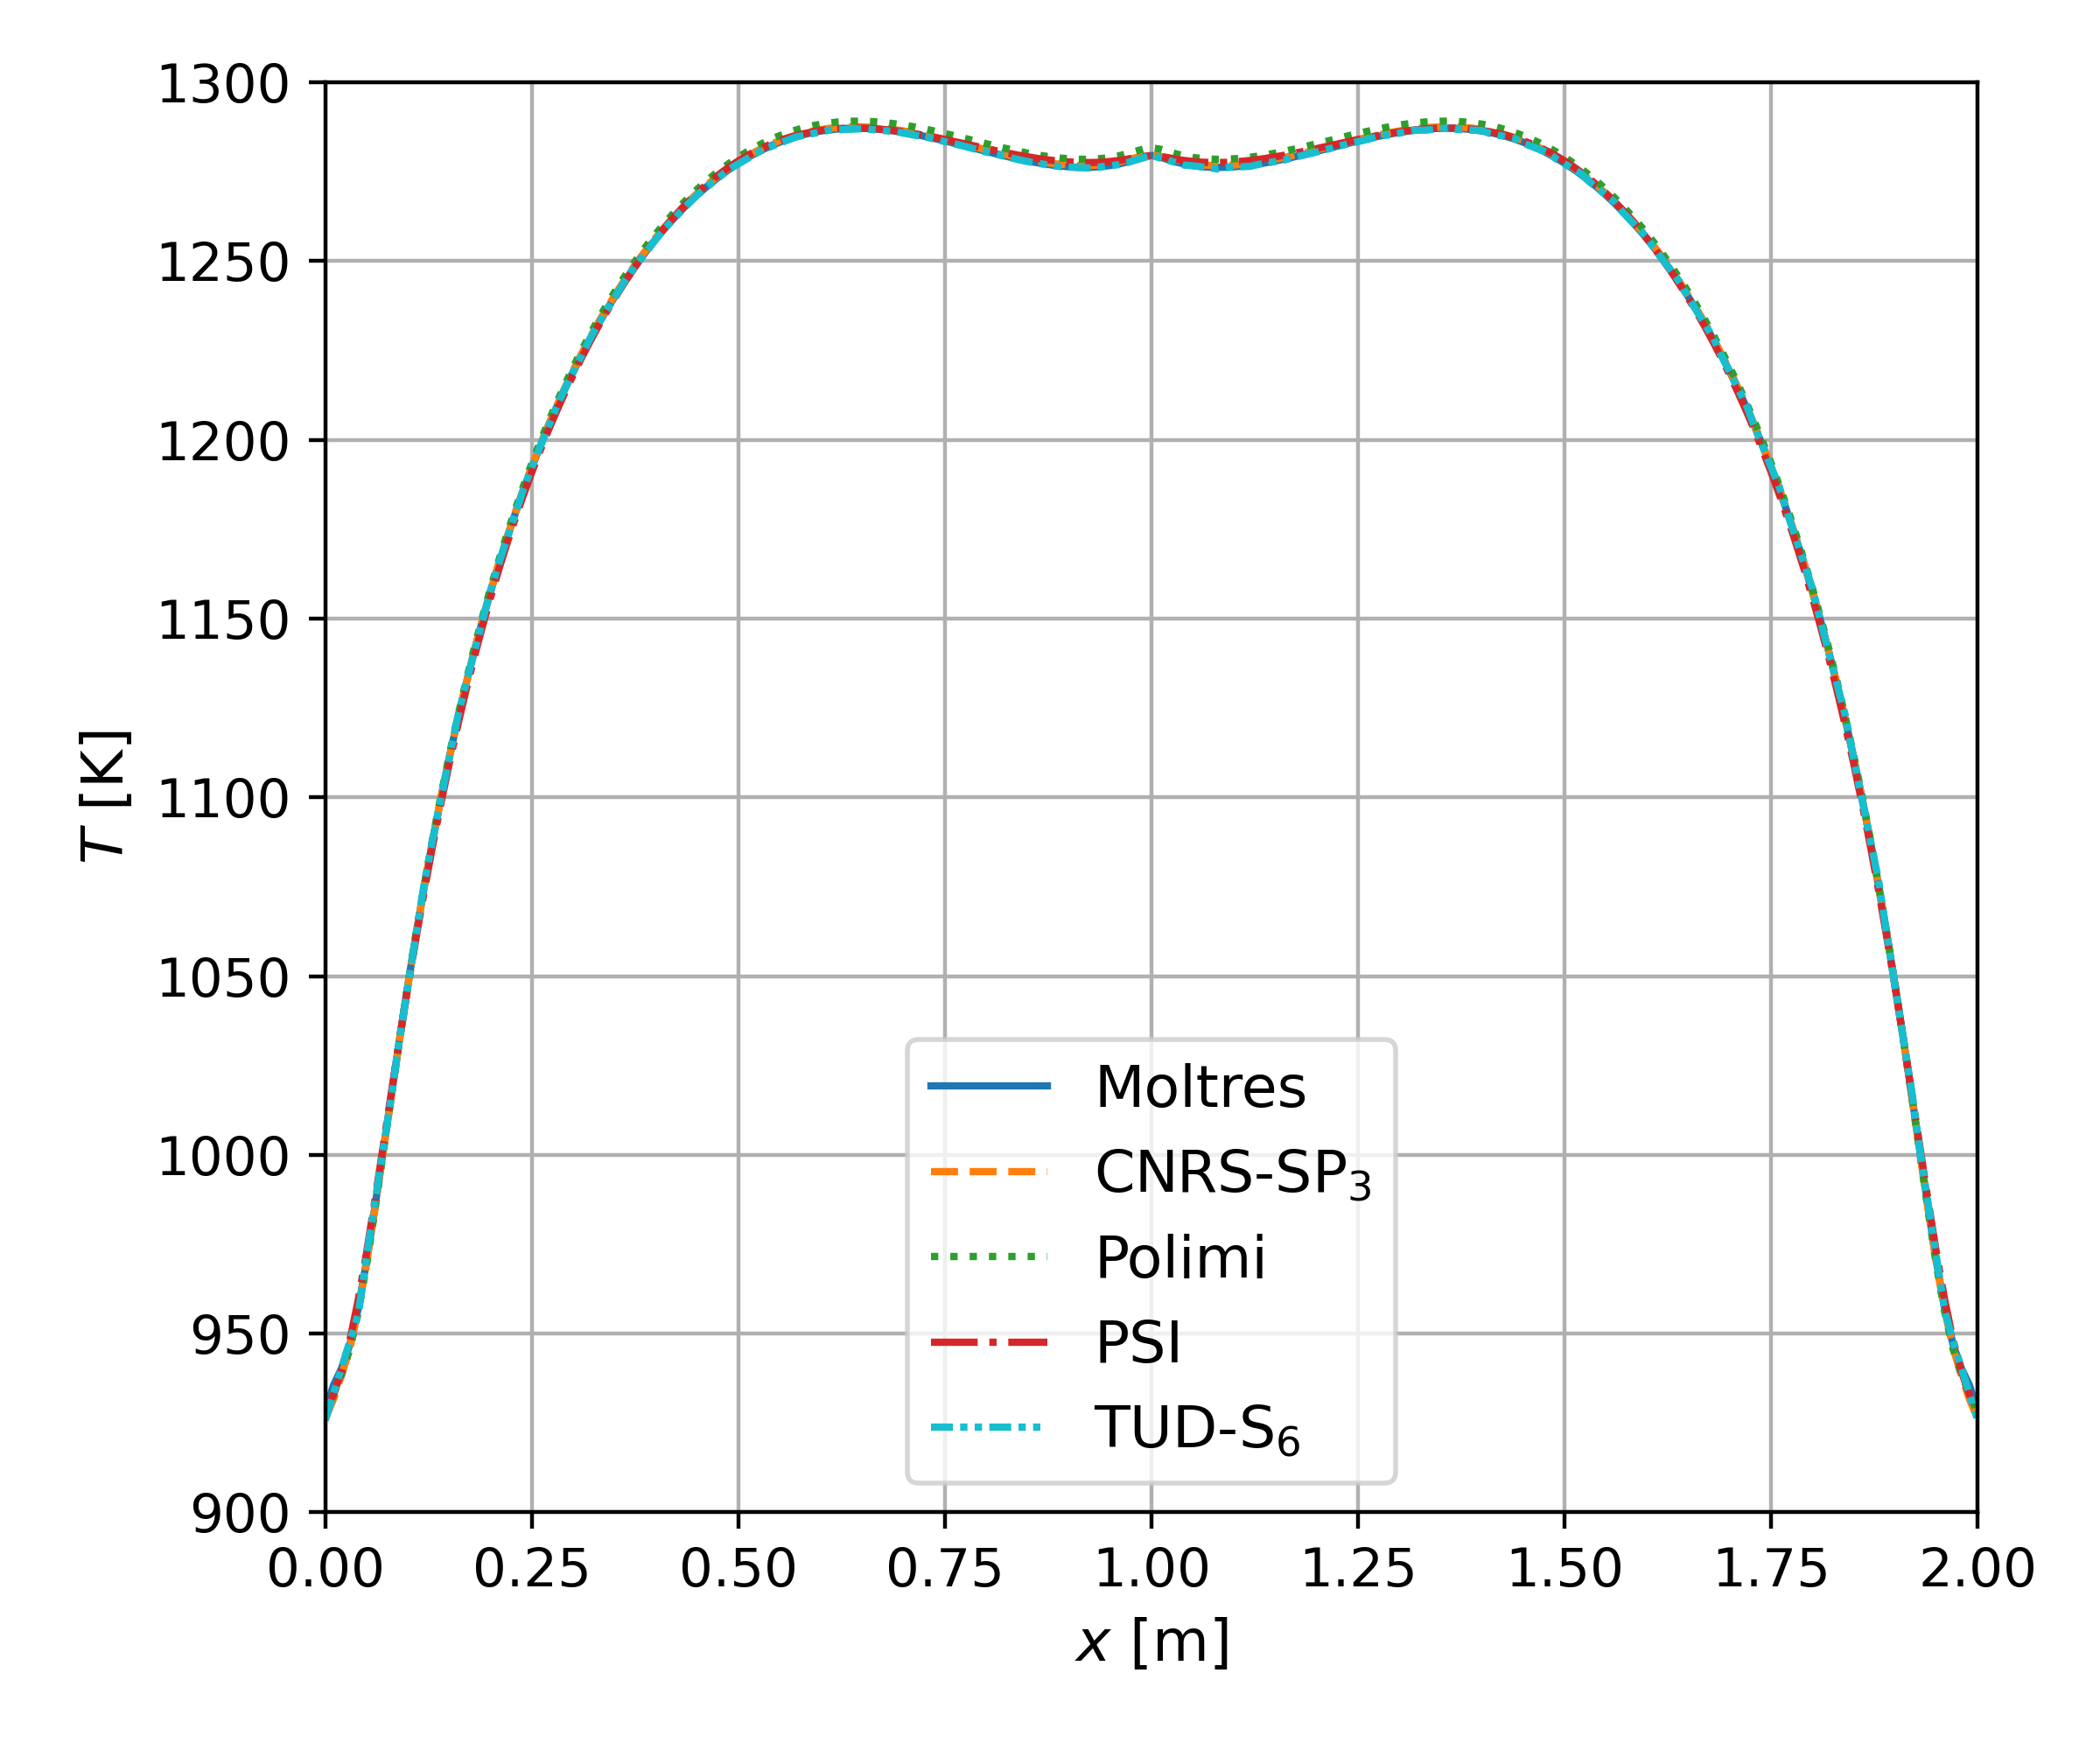
\includegraphics[width=.49\columnwidth]{1-3-temp-plot}
	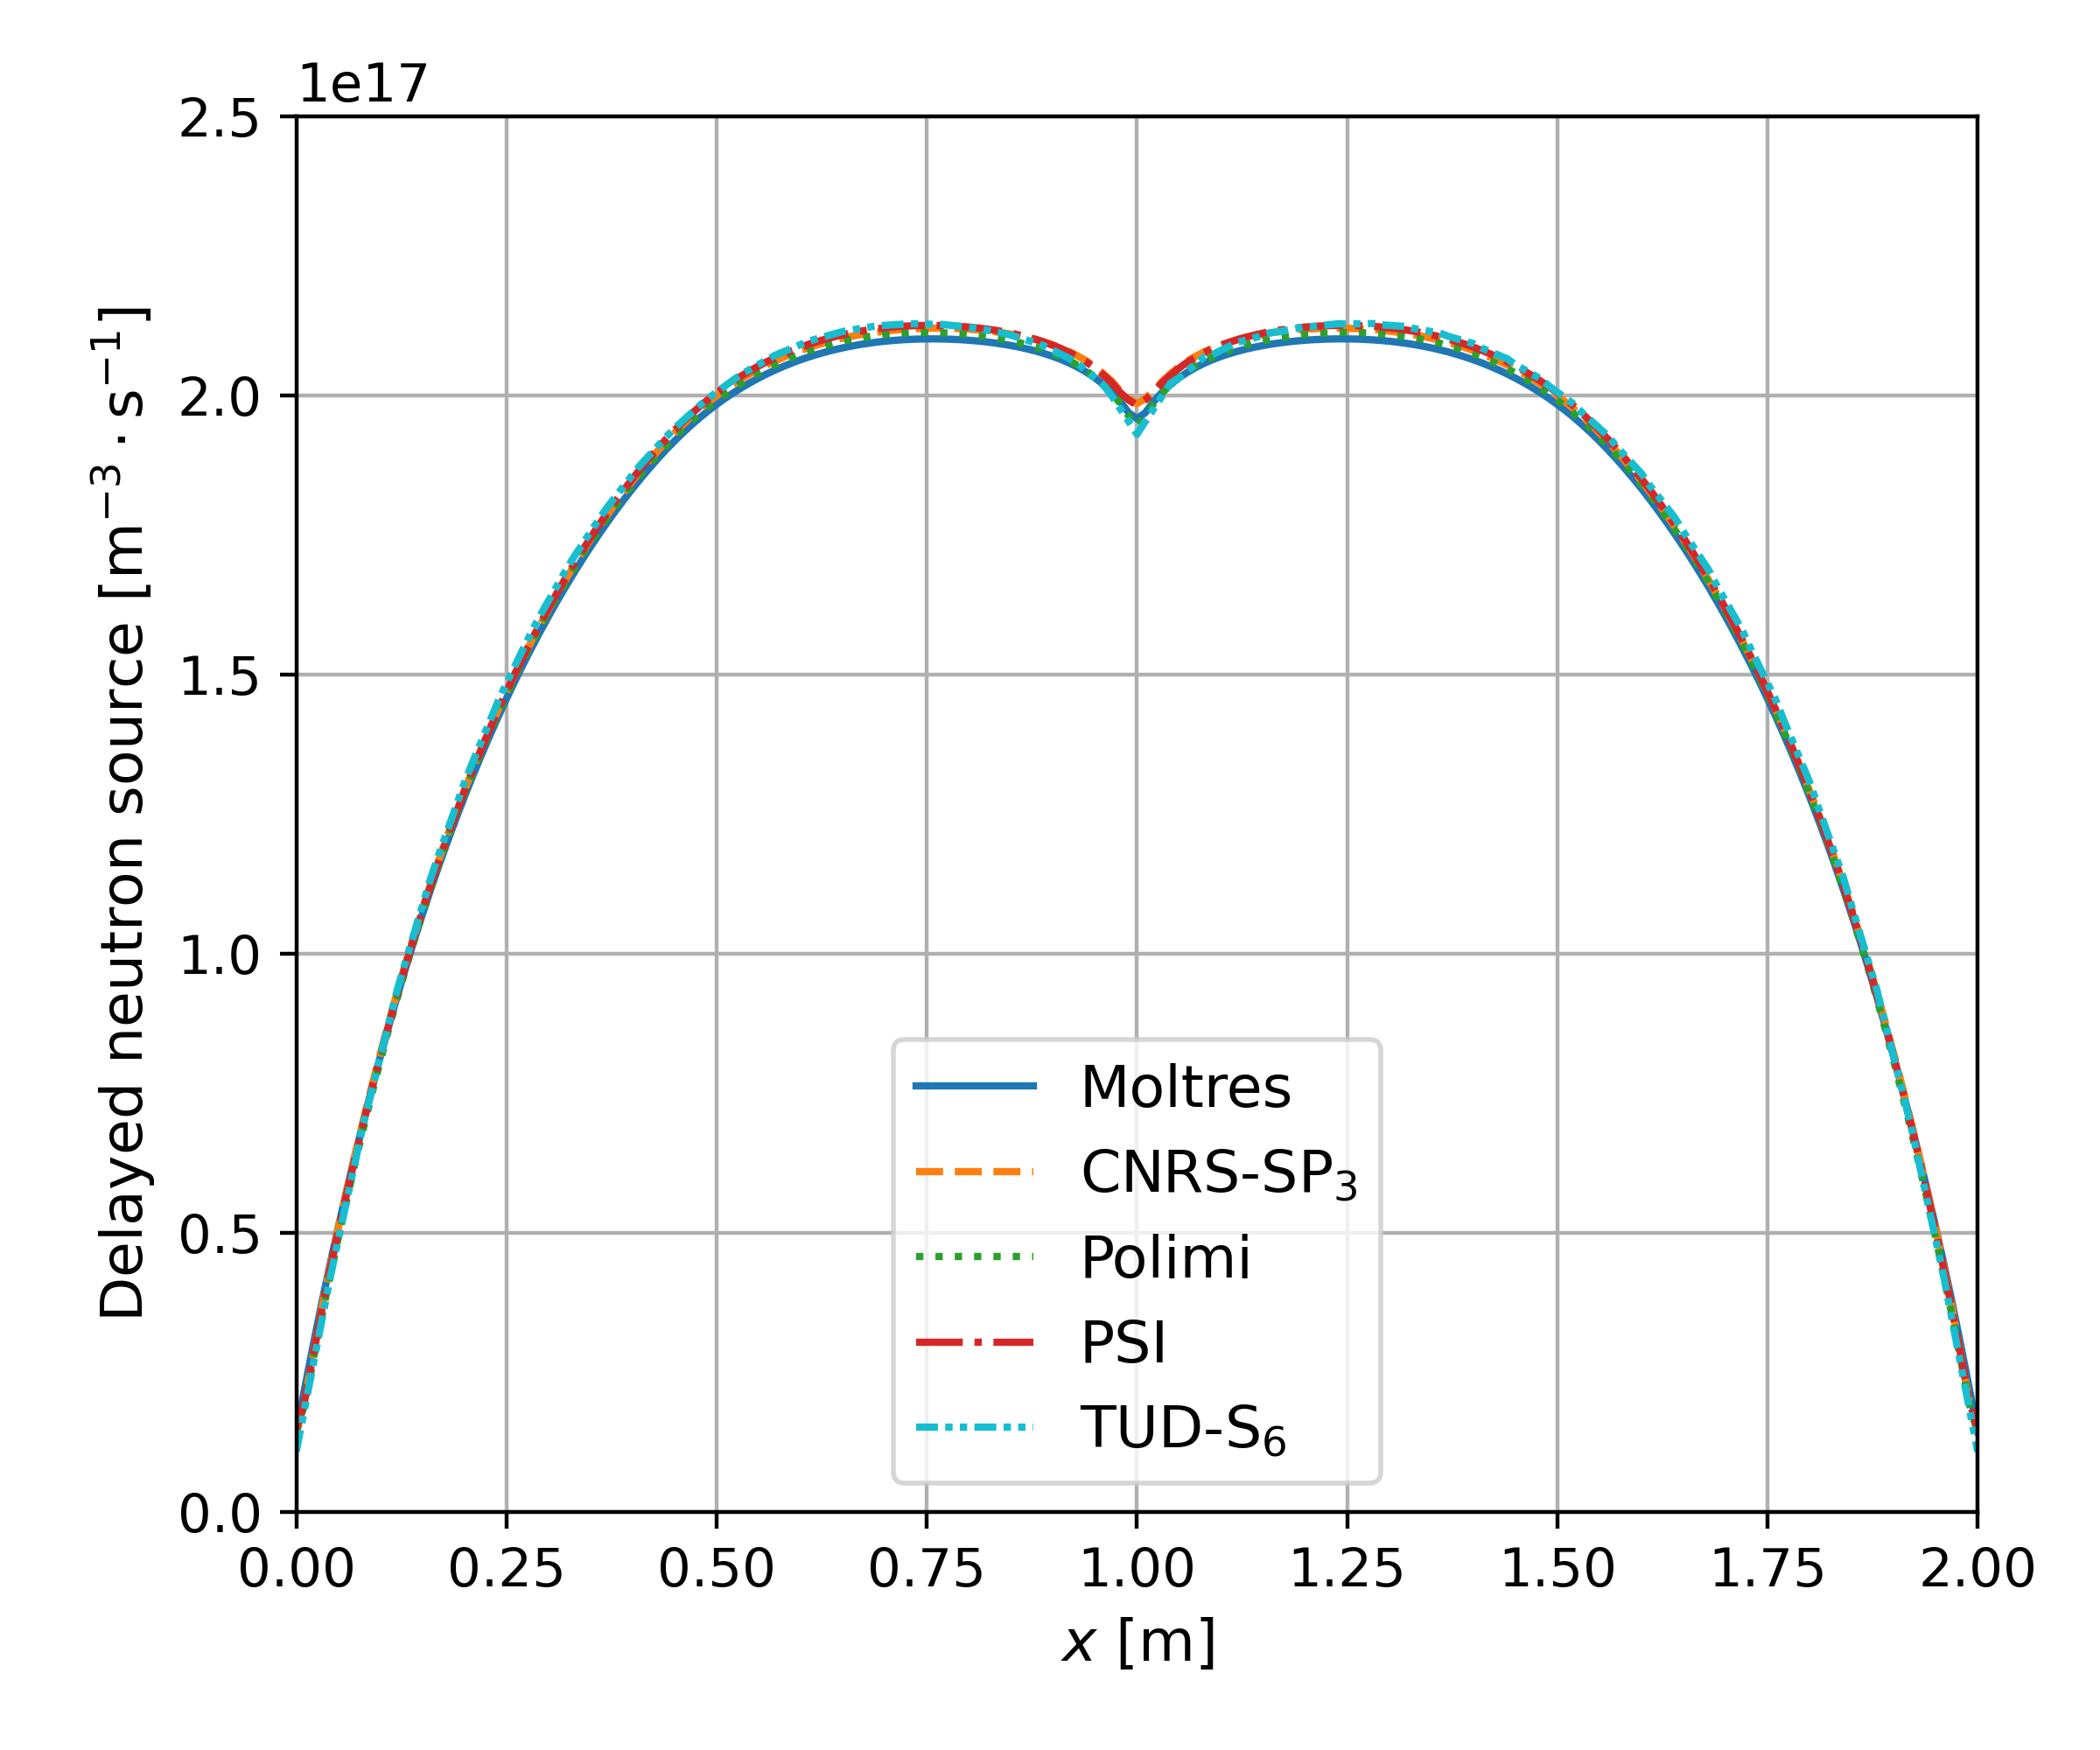
\includegraphics[width=.49\columnwidth]{1-3-dnp-plot}
	\caption{Step 1.3 \textemdash\ Vertical velocity component, temperature distribution,
	and delayed neutron source along AA'.}
	\label{fig:1.3}
\end{figure}

\FloatBarrier

\paragraph{Step 1.4: Full coupling}

Figure \ref{fig:cnrs-color} shows 2D temperature distribution and velocity
streamlines from Moltres for Step 1.4 with $U_{lid} = 0.5$ m$\cdot$s$^{-1}$ and
$P = 1$ GW. Table \ref{table:full} shows the change in $\rho$ under the various
$U_{lid}$ and $P$ values. Refer to Tiberga et al.'s paper
\cite{tiberga_results_2020} for the benchmark participants' corresponding
values. The change in $\rho$ values from Moltres all fall within the range of
benchmark values
for all cases. Furthermore, the $\Delta\rho$ values are all within 1.1 pcm of
the corresponding values from the TUD-S$_2$ model in the benchmark paper. Given
that the $S_2$ discrete ordinates method with isotropic sources is theoretically equivalent to the
multigroup neutron diffusion method, Moltres is largely
consistent with the benchmark participants outside of differences from the
neutronics models.

\begin{figure}[htb]
  \centering
  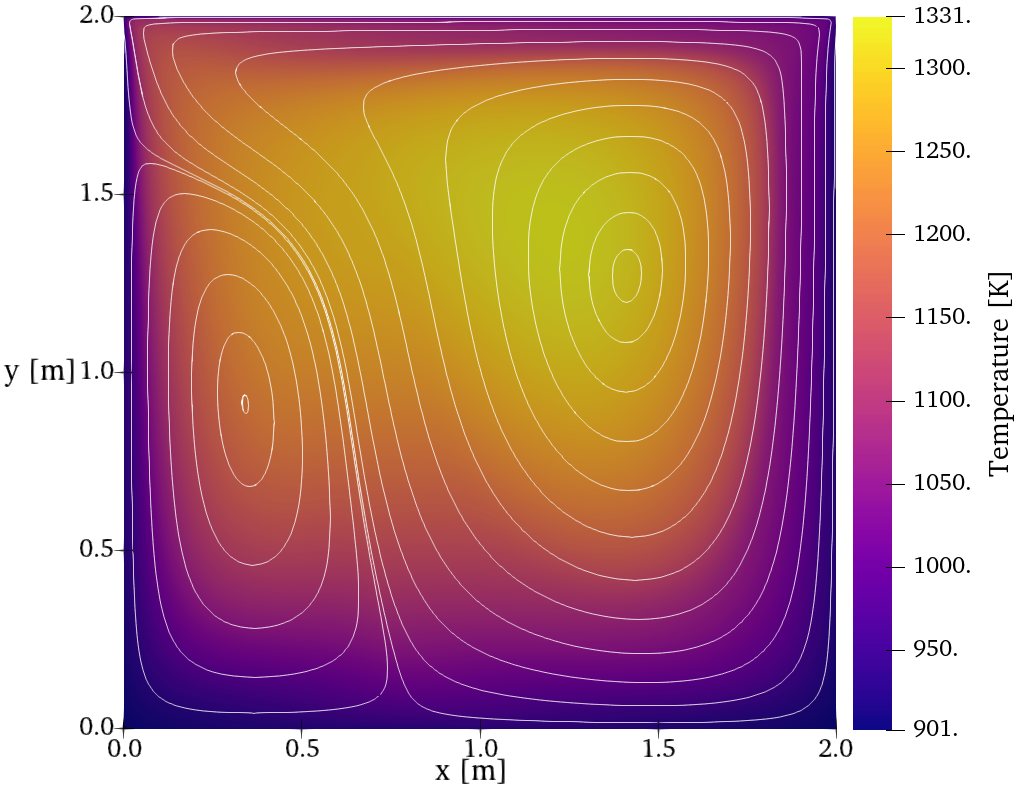
\includegraphics[width=.7\columnwidth]{full-coupled}
  \caption{Temperature distribution from Moltres for the fully coupled
  system (Step 1.4) with buoyancy effects, $P = 1$ GW, and $U_{lid} = 0.5$
  m$\cdot$s$^{-1}$. The lines correspond to the streamlines of the velocity
  field.}
  \label{fig:cnrs-color}
\end{figure}
%
\begin{table}[htb]
	\caption{Reactivity change in Step 1.4, relative to Step 0.2 under various
	$U_{lid}$ and $P$ values.}
	\centering
	\small
	\setlength\tabcolsep{1.5pt}
	\begin{tabular}{c c c c c c}
		\toprule
		& \multicolumn{5}{c}{$\rho_{s1.4} - \rho_{s0.2}$ [pcm]} \\
		\midrule
		{\backslashbox{$U_{lid}$ [m$\cdot$s$^{-1}$]}{$P$ [GW]}} & 0.2 & 0.4 & 0.6 & 0.8 & 1.0 \\
		\midrule
		0.0 & -263.7 & -498.3 & -730.9 & -966.7 & -1207.7 \\
		0.1 & -265.9 & -498.7 & -730.6 & -966.0 & -1206.7 \\
		0.2 & -268.1 & -498.8 & -729.4 & -963.7 & -1203.6 \\
		0.3 & -269.9 & -498.5 & -727.8 & -960.8 & -1199.5 \\
		0.4 & -271.9 & -498.5 & -726.5 & -958.3 & -1195.7 \\
		0.5 & -274.2 & -498.7 & -725.6 & -956.4 & -1192.7 \\
		\bottomrule
	\end{tabular}
	\label{table:full}
\end{table}

\FloatBarrier

\begin{table}[htb]
	\caption{Discrepancy values from Moltres alongside the average and standard
	deviation of the discrepancy values of the benchmark participants for Step
	2.1.}
	\centering
	\small
	\begin{tabular}{l l S S S}
		\toprule
		\multirow{2}{*}{\textbf{Step}} & \multirow{2}{*}{\textbf{Observable}} & {\multirow{2}{*}{\textbf{Moltres [\%]}}} & \multicolumn{2}{c}{\textbf{Benchmark [\%]}} \\
		& & & {Average} & {SD} \\
		\midrule
		\multirow{2}{*}{2.1} & Gain & 0.493 & 0.587 & 0.244 \\
		\cmidrule{2-5}
		& Phase shift & 1.741 & 2.176 & 0.554 \\
		\bottomrule
	\end{tabular}
	\label{table:disc2}
\end{table}
%
\begin{figure}[htb]
	\centering
	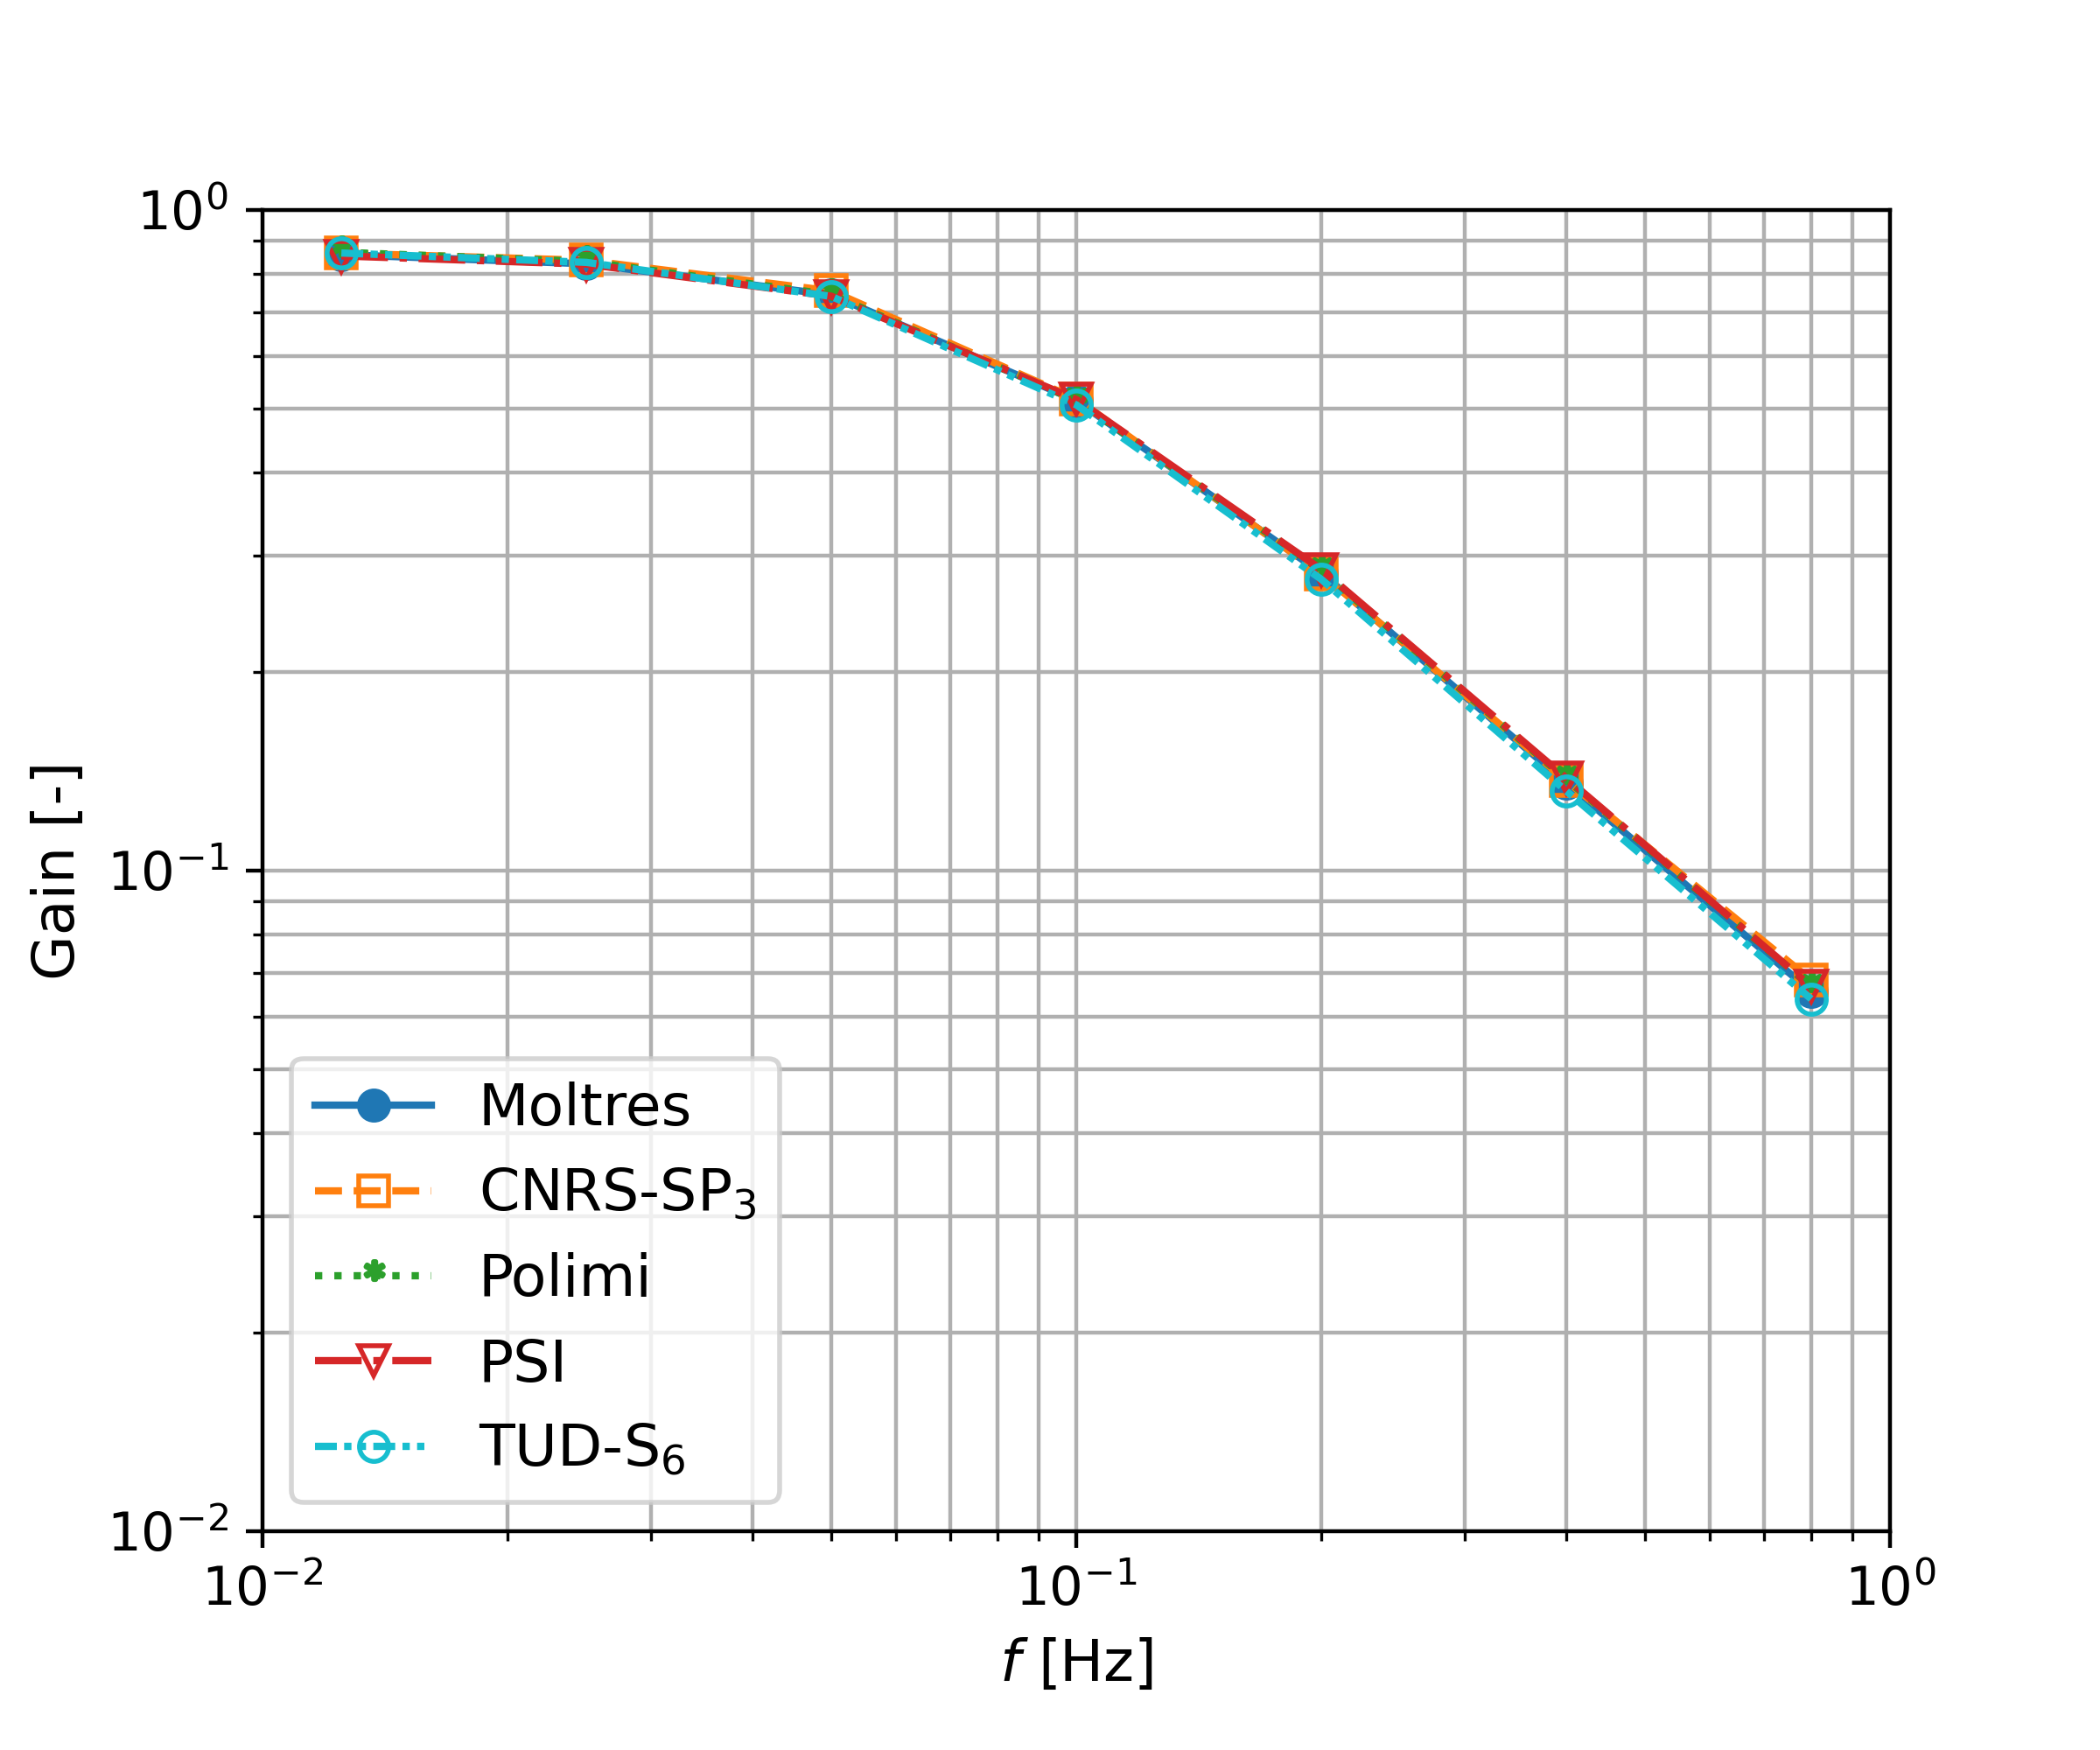
\includegraphics[width=.49\columnwidth]{2-1-gain-plot}
	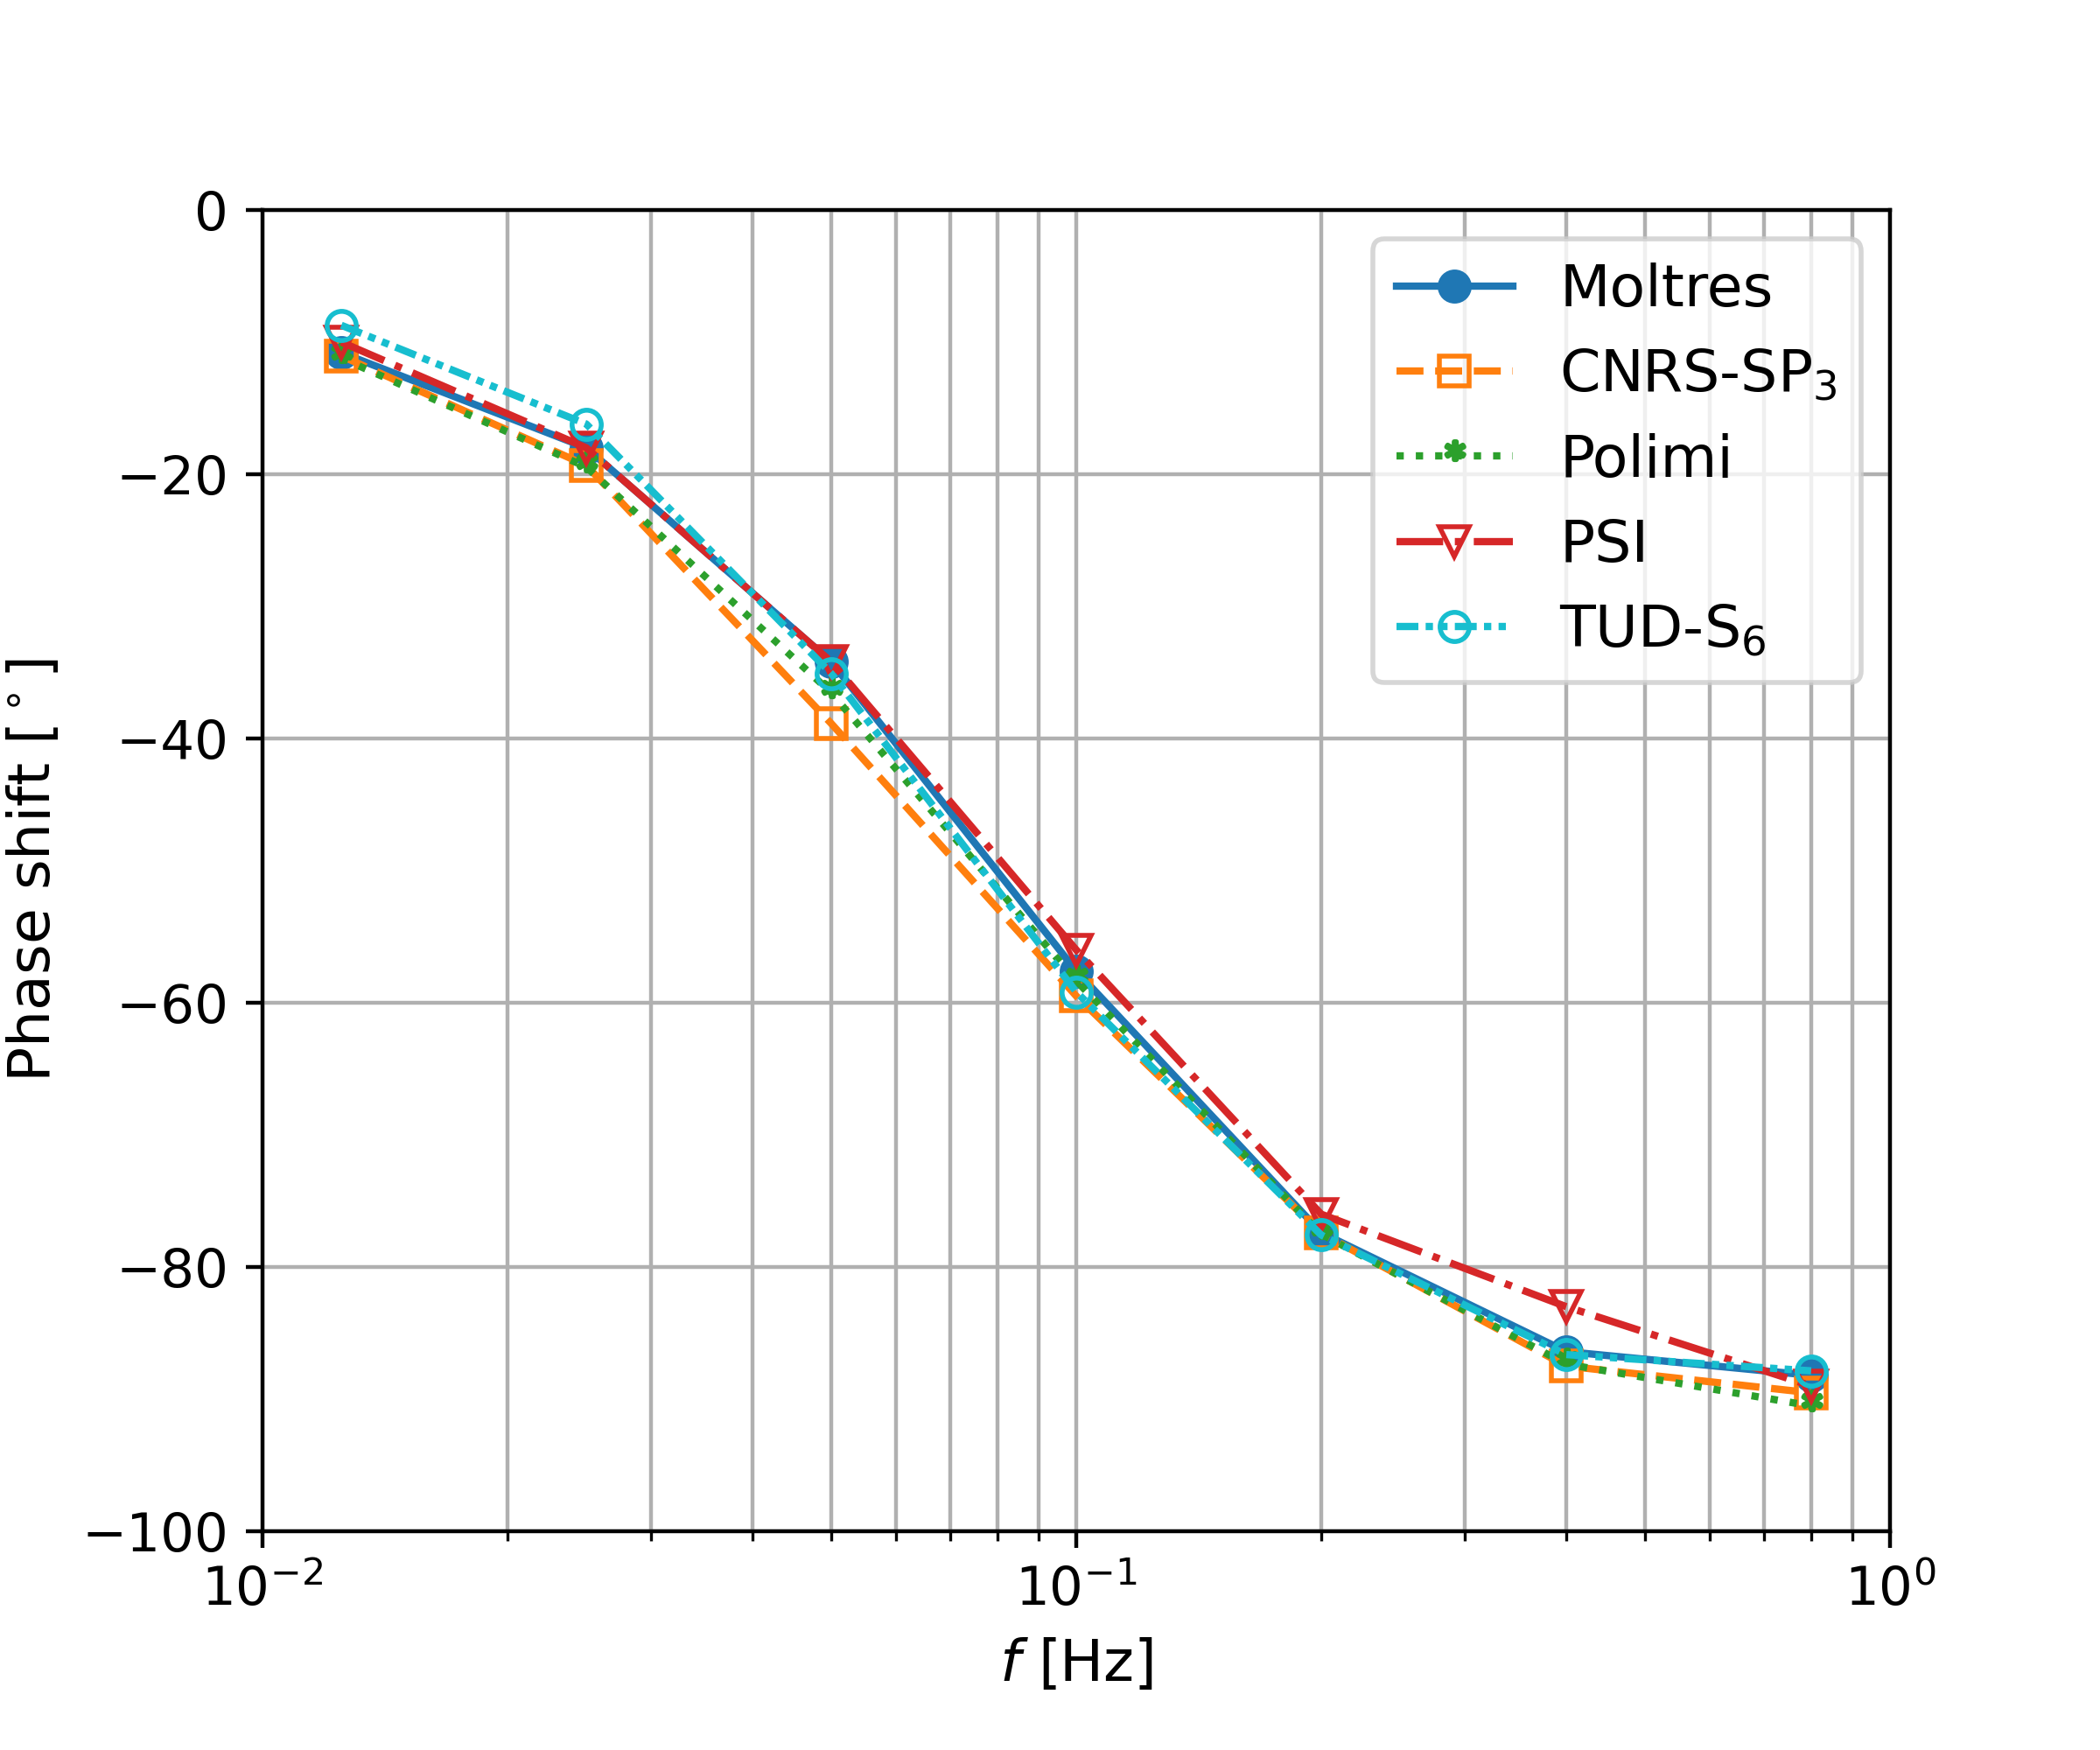
\includegraphics[width=.49\columnwidth]{2-1-phase-plot}
	\caption{Step 2.1 \textemdash\ Bode gain and phase plots of the frequency response of
	the fully coupled system.}
	\label{fig:2.1}
\end{figure}

\subsubsection{Phase 2 results \& discussion}

Lastly, the following subsection discusses the results for the transient cases
in Step 2.1, which involve measuring the response in power output to periodic
perturbations in the heat transfer coefficient.

\paragraph{Step 2.1: Forced convection transient}

Figure \ref{fig:2.1} shows the Bode gain and phase shift plots of the response
in power output in the fully coupled system. Along with the average discrepancy
values from Table \ref{table:disc2}, the results show that Moltres is
consistent with the benchmark. The gain data points from all \gls{MSR} software
agree closely with one another. Moltres reports an average discrepancy value of
0.496\%, slightly lower than the benchmark average of 0.587\%. On the other
hand, the phase shift data points show a greater spread over the various driving
frequencies. We note the different timestepping schemes and timestep
sizes among the different software packages, which is likely responsible for
the variations in the phase shift. Even with a precision of
$\pm0.9^\circ$ for each phase shift value, Moltres accurately reproduces the
correct trend with a lower average discrepancy (1.741\%) than the benchmark
participants' average (2.176\%).

\FloatBarrier

\subsection{Summary}

\glspl{MSR} feature significant multiphysics interactions, presenting
computational challenges for many existing multiphysics reactor analysis
software. This chapter presents code-to-code verification of Moltres'
capabilities in modeling such multiphysics phenomena in fast-spectrum
\glspl{MSR} based on the CNRS benchmark \cite{tiberga_results_2020}.
The CNRS benchmark assesses multiphysics \gls{MSR} simulation
software through several steps involving single-physics and coupled
neutronics/thermal-hydraulics problems.

The results showed that Moltres is consistent with the participating software
presented in the CNRS benchmark paper for modeling important phenomena
in fast-spectrum \glspl{MSR}. The percentage discrepancies in the various
neutronics, velocity, and temperature quantities mostly fall below or within
one standard deviation of the average of the benchmark participants.
Minor deviations in the temperature in Steps 0.3 and 1.2 
stem from the discontinuous velocity
boundaries on the top corners in the lid-driven cavity flow. We have shown that
these deviations are limited to the top boundary of the domain and do not
affect the rest of the physical parameters. The results from
Moltres agree closest with the TUD-S$_2$ software package, which implements the
$S_2$ discrete ordinates method for
neutron transport on a uniform structured mesh with a \gls{DFEM}-based solver.
These features make Moltres the most similar to the TUD-$S_2$ model as compared
to the other models, which employ different neutron transport models,
non-uniform meshes, or finite volume-based solvers.

This work verifies Moltres' capabilities for future work involving the modeling and
simulation of fast-spectrum \glspl{MSR} such as the European \gls{MSFR} and
TerraPower's \gls{MCFR} \cite{terrapower_terrapower_2021}. Notably, the CNRS
benchmark does not assess modeling capabilities for complex physics phenomena
such as turbulent flow in \glspl{MSR}. However, we expect coolant loops in many \gls{MSR} designs
will experience turbulent flow under regular operation or accident scenarios.
These expectations, alongside the subpar results of pump-initiated accidents
reported in Section \ref{sec:msfr}, call for the implementation and
verification of a turbulence model in Moltres to accurately model \glspl{MSR}.

\FloatBarrier

